\documentclass[a4paper]{article}

\input{style/ch_xelatex.tex}
\input{style/scala.tex}

\usepackage{ctex}
\usepackage{amsmath,amssymb,bm}
\usepackage{geometry}
\usepackage{graphicx}
\usepackage{xcolor}
\usepackage{caption}
\usepackage{float}
\usepackage{booktabs,tabularx,longtable,multirow}
\usepackage{enumerate}
\usepackage{listings}
\usepackage{algorithm}
\usepackage{algorithmicx}
\usepackage{algpseudocode}
\usepackage{lastpage}
\usepackage{fancyhdr}
\usepackage{hyperref}
\usepackage{tikz}
\usepackage{pgfplots}
\usetikzlibrary{arrows.meta,positioning,shapes.geometric,calc}
\pgfplotsset{compat=1.18}

\geometry{a4paper,left=2.3cm,right=2.3cm,top=2.7cm,bottom=2.7cm}
\hypersetup{colorlinks=true,linkcolor=black,urlcolor=blue,citecolor=black}
\setcounter{secnumdepth}{4}
\setcounter{tocdepth}{3}

\lstset{
  breaklines=true,
  basicstyle=\small\ttfamily,
  keywordstyle=\color{blue!70}\bfseries,
  commentstyle=\color{red!50!green!50!blue!50},
  stringstyle=\ttfamily,
  extendedchars=false,
  linewidth=\textwidth,
  numbers=left,
  numberstyle=\tiny\color{blue!50},
  frame=single
}

\floatname{algorithm}{Algorithm}
\renewcommand{\algorithmicrequire}{\textbf{Input:}}
\renewcommand{\algorithmicensure}{\textbf{Output:}}
\makeatletter
\newenvironment{breakablealgorithm}
  {\begin{center}\refstepcounter{algorithm}\hrule height.8pt depth0pt \kern2pt
   \renewcommand{\caption}[2][\relax]{{\raggedright\textbf{\ALG@name~\thealgorithm} ##2\par}
   \ifx\relax##1\relax\addcontentsline{loa}{algorithm}{\protect\numberline{\thealgorithm}##2}\else\addcontentsline{loa}{algorithm}{\protect\numberline{\thealgorithm}##1}\fi
   \kern2pt\hrule\kern2pt}}
  {\kern2pt\hrule\relax\end{center}}
\makeatother

\pagestyle{fancy}
\lhead{\kaishu \leftmark}
\rhead{\kaishu 并行程序设计期末报告}
\lfoot{}
\cfoot{\thepage\ of \pageref{LastPage}}
\rfoot{}
\renewcommand{\headrulewidth}{0.1pt}
\renewcommand{\footrulewidth}{0pt}

\renewcommand{\contentsname}{目录}
\renewcommand{\figurename}{图}
\renewcommand{\tablename}{表}
\renewcommand{\refname}{参考文献}
\newcommand{\ip}[2]{\left\langle #1,#2 \right\rangle}
\newcommand{\dist}[2]{1-\ip{#1}{#2}}
\newcommand{\bigO}[1]{O\!\left(#1\right)}
\newcommand{\deep}{DEEP100K}

\tikzset{
  flowstart/.style={rectangle, rounded corners, draw=black, fill=blue!10, align=center, minimum width=3.0cm, minimum height=0.75cm},
  flowproc/.style={rectangle, draw=black, fill=gray!10, align=center, minimum width=3.0cm, minimum height=0.75cm},
  flowidx/.style={rectangle, draw=black, fill=orange!12, align=center, minimum width=2.7cm, minimum height=0.7cm},
  floweval/.style={rectangle, rounded corners, draw=black, fill=green!12, align=center, minimum width=3.0cm, minimum height=0.75cm},
  flowarrow/.style={-{Stealth[length=2mm]}, thick}
}

\begin{document}

\begin{titlepage}
\begin{center}

\includegraphics[width=0.78\textwidth]{NKU.png}\\[1cm]
\vspace{18mm}
{\Huge\bfseries\kaishu 计算机学院}\\[0.8cm]
{\Huge\bfseries\kaishu 并行程序设计期末报告}\\[2cm]
{\huge\bfseries\kaishu ANN}\\[0.6cm]
{\huge\bfseries\kaishu 近似最近邻搜索算法}\\[2cm]
\vfill
{\Large\kaishu 姓名：刘宇泽}\\[0.5cm]
{\Large\kaishu 学号：2411334}\\[0.5cm]
{\Large\kaishu 专业：计算机科学与技术}\\[1.2cm]
{\Large 2026 年 7 月 1 日}
\end{center}
\end{titlepage}

\clearpage
\tableofcontents
\clearpage
\setcounter{page}{1}

\section{系统全流程综述}

\subsection{问题定义与评估指标}

近似最近邻搜索（Approximate Nearest Neighbor Search, ANNS）的目标是在高维向量集合中快速找到与查询向量最接近的若干个向量。给定 base 向量集合
\[
X=\{x_1,x_2,\dots,x_N\},\quad x_i\in \mathbb{R}^{d},
\]
以及查询向量 $q\in \mathbb{R}^{d}$，精确 $k$ 近邻搜索要求返回集合 $S$，满足 $|S|=k$ 且
\[
\forall x\in S,\ \forall y\notin S,\quad \delta(x,q) < \delta(y,q).
\]
本学期实验中使用的主要距离形式为内积距离：
\[
\delta(x,q)=1-\ip{x}{q}=1-\sum_{j=1}^{d}x_jq_j.
\]
ANNS 不要求结果完全等于精确 Top-$k$，而是在保持较高召回率的前提下降低查询延迟。因此所有实验围绕两个核心指标展开：
\[
\mathrm{Recall@}k=\frac{|K_{NN}(q)\cap K_{ANN}(q)|}{k},
\qquad
\mathrm{Latency}=\frac{\mathrm{Total\ Query\ Time}}{\mathrm{Query\ Count}}.
\]

\subsection{数据集与 Base 数据预处理}

所有实验均围绕 \deep 数据集展开，数据规模如表\ref{tab:dataset}所示。该数据集的 base 与 query 均以 fbin 二进制格式存储，读取后在内存中组织为连续的 row-major \texttt{float*} 数组，每 96 个 float 表示一个向量。ground truth 文件保存每条 query 的精确 Top-100 近邻编号，用于计算 Recall@10。

\begin{table}[H]
\centering
\caption{\deep 数据集规模}
\label{tab:dataset}
\begin{tabular}{lccc}
\toprule
文件 & 内容 & 规模 & 维度 \\
\midrule
\texttt{DEEP100K.base.100k.fbin} & base 向量 & 100000 & 96 \\
\texttt{DEEP100K.query.fbin} & query 向量 & 10000 & 96 \\
\texttt{DEEP100K.gt.query.100k.top100.bin} & ground truth & 10000$\times$100 & - \\
\bottomrule
\end{tabular}
\end{table}

Base 数据预处理的核心目的不是改变原始语义，而是为后续索引结构和并行访问建立更适合的内存布局。不同算法对应的预处理方式不同，如表\ref{tab:index-structures}所示。

\begin{table}[H]
\centering
\small
\caption{Base 数据预处理与索引结构}
\label{tab:index-structures}
\begin{tabularx}{\textwidth}{lXlX}
\toprule
算法 & 离线预处理 / 索引构建 & 主要参数 & 在线查询对象 \\
\midrule
Flat & 不建立额外索引，保留原始 float32 base 数组 & - & 全量 base 向量 \\
SQ & 按维度计算均值与缩放因子，将 float32 编码为 uint8 & 候选数 $p$ & 量化码粗排 + 原始向量精排 \\
PQ & 将向量划分为 $M$ 个子空间，分别 KMeans 得到码本并编码 & $M$, ksub, $p$ & LUT 查表粗排 + 原始向量精排 \\
IVF & 对 base 聚类，保存 centroid 与倒排链表，可按簇重排内存 & nlist, nprobe & 最近 nprobe 个倒排链表 \\
HNSW & 构建分层近邻图或底层近邻图 & $M$, efConstruction, ef & 图搜索候选队列 \\
MPI 分片 & 按 rank 对 base 连续切分，每个进程构建局部索引 & world size & 局部 Top-$k$ 后全局 merge \\
GPU batch & 将 base 或候选 id 上传显存，query 按 batch 组织 & batch size & 距离矩阵或有效 pair \\
\bottomrule
\end{tabularx}
\end{table}

从全流程角度看，以上索引结构并不是互斥优化，而是分别作用在不同成本项上。对单条 query，可将端到端延迟近似拆分为
\[
T_{\mathrm{query}}\approx
T_{\mathrm{candidate}}+
T_{\mathrm{distance}}+
T_{\mathrm{topk}}+
T_{\mathrm{comm}}+
T_{\mathrm{transfer}}.
\]
其中 $T_{\mathrm{candidate}}$ 表示候选产生成本，$T_{\mathrm{distance}}$ 表示候选距离计算成本，$T_{\mathrm{topk}}$ 表示堆维护与归并成本，$T_{\mathrm{comm}}$ 主要出现在 MPI 阶段，$T_{\mathrm{transfer}}$ 主要出现在 GPU 阶段。平时各实验可以按表\ref{tab:cost-decomposition}统一理解。

\begin{table}[H]
\centering
\scriptsize
\caption{ANNS 全流程成本项与平时实验的对应关系}
\label{tab:cost-decomposition}
\begin{tabularx}{\textwidth}{lXlX}
\toprule
成本项 & 主要来源 & 对应实验 & 优化后的新瓶颈 \\
\midrule
$T_{\mathrm{candidate}}$ & IVF 选簇、HNSW 图扩展、PQ 粗排候选生成 & IVF 的 nprobe、HNSW 的 ef、PQ 的 $p$ 参数扫描 & recall 与候选规模之间的 trade-off \\
$T_{\mathrm{distance}}$ & 内积或 L2 距离计算，占 Flat 与精排阶段主要时间 & SIMD NEON、OpenMP/Pthread 扫描、GPU kernel & 访存带宽、寄存器占用与线程粒度 \\
$T_{\mathrm{topk}}$ & 每条 query 的局部堆维护、线程局部结果归并 & Flat、PQ、IVF 的 Top-$k$ / Top-$p$ merge & 候选数增大后堆操作占比上升 \\
$T_{\mathrm{comm}}$ & query 广播、各 rank 局部结果收集、全局 merge & MPI-IVF、分片 HNSW、IVF+HNSW & 分片负载不均衡和跨 shard 图信息缺失 \\
$T_{\mathrm{transfer}}$ & H2D 输入上传、D2H 距离矩阵或候选结果回传 & GPU Flat Batch、IVF Union、IVF Compact & D2H 结果规模和 host 端选择开销 \\
\bottomrule
\end{tabularx}
\end{table}

因此，后文的对比不只讨论某个 kernel 或某个线程数是否更快，而是分析每种并行方法到底压缩了哪个成本项，以及它是否把瓶颈转移到了新的位置。例如 SIMD 主要降低 $T_{\mathrm{distance}}$，但不会减少访问向量数量；IVF/HNSW 主要降低 $T_{\mathrm{candidate}}$ 与 $T_{\mathrm{distance}}$ 的输入规模；GPU Compact 进一步降低 $T_{\mathrm{transfer}}$，避免把大量无效 pair 的距离结果回传到 CPU。

\subsection{端到端流程}

一个完整 ANNS 系统可以分为离线阶段和在线阶段。离线阶段负责读取数据、预处理与索引构建；在线阶段负责接收 query、执行搜索、维护 Top-$k$ 并计算 recall/latency。图\ref{fig:system-flow}给出了本报告统一采用的系统流程。

\begin{figure}[H]
\centering
\begin{tikzpicture}[node distance=0.85cm]
\node[flowstart] (load) {读取 \deep 数据};
\node[flowproc, below=of load] (pre) {Base 预处理};
\node[flowidx, below left=0.8cm and 2.0cm of pre] (flat) {Flat\\原始数组};
\node[flowidx, below left=0.8cm and 0.3cm of pre] (pq) {SQ / PQ\\量化编码};
\node[flowidx, below right=0.8cm and 0.3cm of pre] (ivf) {IVF\\倒排链表};
\node[flowidx, below right=0.8cm and 2.0cm of pre] (hnsw) {HNSW\\近邻图};
\node[flowproc, below=2.0cm of pre] (query) {在线 query 到达};
\node[flowproc, below=of query] (search) {粗排 / 图搜索 / batch 打分};
\node[flowproc, below=of search] (rerank) {候选集合精排与 Top-$k$ merge};
\node[floweval, below=of rerank] (eval) {与 ground truth 比较\\计算 Recall@10 与 Latency};
\draw[flowarrow] (load) -- (pre);
\draw[flowarrow] (pre) -- (flat);
\draw[flowarrow] (pre) -- (pq);
\draw[flowarrow] (pre) -- (ivf);
\draw[flowarrow] (pre) -- (hnsw);
\draw[flowarrow] (flat) |- (query);
\draw[flowarrow] (pq) |- (query);
\draw[flowarrow] (ivf) |- (query);
\draw[flowarrow] (hnsw) |- (query);
\draw[flowarrow] (query) -- (search);
\draw[flowarrow] (search) -- (rerank);
\draw[flowarrow] (rerank) -- (eval);
\end{tikzpicture}
\caption{ANNS 系统端到端流程}
\label{fig:system-flow}
\end{figure}

离线索引构建阶段决定了在线阶段能够访问哪些候选以及以何种内存布局访问。平时实验中虽然各算法代码分散在 SIMD、Pthread/OpenMP、MPI、GPU 几个实验目录下，但其构建逻辑可以统一为算法\ref{alg:index-build}。

\begin{breakablealgorithm}
\caption{Base 数据预处理与索引构建}
\label{alg:index-build}
\begin{algorithmic}[1]
\Require base 向量文件 $X$，算法类型 $A$，参数集合 $\theta$
\Ensure 可供在线查询使用的索引结构 $\mathcal{I}$
\State 读取 \texttt{fbin} 文件，将 $N\times d$ 个 float 组织为连续 row-major 数组
\State 保留原始 base 数组 $X_{\mathrm{raw}}$，用于 Flat 精确扫描或量化方法的 rerank
\If{$A=\mathrm{Flat}$}
  \State $\mathcal{I}\gets X_{\mathrm{raw}}$
\ElsIf{$A=\mathrm{SQ}$}
  \State 按维度统计缩放参数，将 float32 编码为 uint8 量化码
  \State $\mathcal{I}\gets$ 量化码数组、缩放参数与原始 base 指针
\ElsIf{$A=\mathrm{PQ}$}
  \State 将 $d$ 维向量划分为 $M$ 个子空间，在每个子空间训练码本
  \State 为每个 base 向量记录 $M$ 个子空间码字编号，查询时构造 LUT
  \State $\mathcal{I}\gets$ PQ 码本、编码数组与 rerank 所需原始 base
\ElsIf{$A=\mathrm{IVF}$}
  \State 对 base 聚类得到 nlist 个 centroid，并将每个向量分配到最近 centroid
  \State 按倒排链表重排 id 与向量，记录每个 list 的起止 offset
  \State $\mathcal{I}\gets$ centroids、list offsets、倒排 id 与 list 内向量
\ElsIf{$A=\mathrm{HNSW}$}
  \State 按 efConstruction 与 $M$ 插入节点，维护分层邻接表或底层邻接表
  \State $\mathcal{I}\gets$ 图入口点、层级信息与邻接边
\ElsIf{$A=\mathrm{MPI}$}
  \State 按 rank 切分 base，每个 rank 在本地重复执行 Flat/IVF/HNSW 构建
  \State $\mathcal{I}\gets$ 局部索引与全局 id 偏移
\ElsIf{$A=\mathrm{GPU}$}
  \State 将 base、centroid、offset 或候选 id 数组拷贝到 device 端
  \State $\mathcal{I}\gets$ device 指针、batch 参数与 host/device 结果缓冲区
\EndIf
\State \Return $\mathcal{I}$
\end{algorithmic}
\end{breakablealgorithm}

该伪代码也解释了为什么同样是 ANNS，离线阶段的成本差异很大：Flat 基本没有构建成本，IVF 需要聚类和倒排组织，PQ 需要训练码本和编码，HNSW 则需要构图。本文的 latency 主要统计在线查询，但在方案选择时仍会把离线构建复杂度作为分析维度。

\subsection{查询搜索逻辑}

本学期实验覆盖了从精确搜索到近似搜索的多种算法。它们的共同结构可以抽象为：先生成候选集合，再对候选进行 Top-$k$ 选择；不同算法的主要差异在于候选集合如何产生，以及候选距离是精确计算还是近似计算。

\begin{breakablealgorithm}
\caption{统一 ANNS 查询流程}
\begin{algorithmic}[1]
\Require base 数据或索引结构 $\mathcal{I}$，查询向量 $q$，近邻数 $k$
\Ensure Top-$k$ 结果集合 $R$
\State 根据算法类型选择候选生成方式
\If{Flat}
  \State candidates $\gets$ all base vectors
\ElsIf{SQ / PQ}
  \State 使用量化码或 LUT 进行粗排，取 Top-$p$ 候选
\ElsIf{IVF}
  \State 计算 $q$ 到 centroid 的距离，选择最近 nprobe 个倒排链表
\ElsIf{HNSW}
  \State 从入口点出发维护候选队列，按 ef 控制搜索宽度
\EndIf
\State 对 candidates 进行距离计算或精排
\State 维护大小为 $k$ 的堆，得到 Top-$k$
\State \Return $R$
\end{algorithmic}
\end{breakablealgorithm}

从工程实现角度看，Top-$k$ 维护通常采用大小为 $k$ 或 $p$ 的堆。多线程和 MPI 版本中，每个线程或 rank 先维护局部 Top-$k$ / Top-$p$，最后由主线程或 rank0 做多路归并。GPU 版本中，当前实现主要在 GPU 上完成距离打分，Top-$k$ 选择仍在 CPU 侧完成，因此 Device-to-Host 距离结果回传成为重要瓶颈。

\subsection{召回率评估机制}

评估阶段对每条 query 读取 ground truth 的前 $k$ 个编号，与算法返回的 $k$ 个编号求交集，再对所有 query 取平均。图\ref{fig:eval-flow}给出了评估逻辑。

\begin{figure}[H]
\centering
\begin{tikzpicture}[node distance=0.85cm]
\node[flowstart] (ann) {算法返回 Top-$k$};
\node[flowproc, below left=0.8cm and 1.8cm of ann] (gt) {读取 ground truth Top-$k$};
\node[flowproc, below right=0.8cm and 1.8cm of ann] (lat) {记录 query 时间};
\node[flowproc, below=1.7cm of ann] (inter) {计算集合交集};
\node[floweval, below=of inter] (avg) {平均 Recall@10 / Latency};
\draw[flowarrow] (ann) -- (inter);
\draw[flowarrow] (gt) -- (inter);
\draw[flowarrow] (lat) -- (avg);
\draw[flowarrow] (inter) -- (avg);
\end{tikzpicture}
\caption{Recall 与 Latency 评估流程}
\label{fig:eval-flow}
\end{figure}

需要说明的是，本文重点比较在线查询延迟；离线索引构建时间只在分析索引可用性时讨论。例如 HNSW 查询延迟很低，但构图时间明显高于 Flat 或 IVF，因此更适合查询量足够大的场景。GPU 实验中也单独记录了 build time、kernel time、H2D/D2H time 与 host select time，以区分算法计算和数据传输开销。

\begin{breakablealgorithm}
\caption{Latency-Recall@K 参数扫描与评估}
\label{alg:eval-sweep}
\begin{algorithmic}[1]
\Require 参数集合 $\Theta$，query 集合 $Q$，ground truth $G$，近邻数 $k$
\Ensure 每组配置的 Recall@K 与平均 latency
\ForAll{$\theta\in\Theta$}
  \State 根据 $\theta$ 构建或加载索引 $\mathcal{I}_\theta$
  \State 初始化累计命中数 $hit\gets 0$，累计时间 $time\gets 0$
  \ForAll{$q_i\in Q$}
    \State $t_0\gets$ 当前时间戳
    \State $R_i\gets Search(\mathcal{I}_\theta,q_i,k)$
    \State $t_1\gets$ 当前时间戳
    \State $hit\gets hit+|R_i\cap G_i[1:k]|$
    \State $time\gets time+(t_1-t_0)$
  \EndFor
  \State $\mathrm{Recall@K}(\theta)\gets hit/(|Q|\cdot k)$
  \State $\mathrm{Latency}(\theta)\gets time/|Q|$
  \State 将 $(\mathrm{Recall@K},\mathrm{Latency})$ 写入 CSV 或绘制 trade-off 曲线
\EndFor
\end{algorithmic}
\end{breakablealgorithm}


\section{并行方案对比与 Latency-Recall@K Trade-off}

\subsection{对比原则}

\begin{figure}[H]
\centering
\resizebox{0.98\textwidth}{!}{%
\begin{tikzpicture}[node distance=0.75cm]
\node[flowstart] (data) {DEEP100K\\Base / Query / GT};
\node[flowproc, below=of data] (index) {索引与候选生成层\\Flat / SQ / PQ / IVF / HNSW};
\node[flowidx, below left=1.0cm and 5.3cm of index] (simd) {SIMD\\维度内并行\\距离计算加速};
\node[flowidx, below left=1.0cm and 1.8cm of index] (thread) {OpenMP/Pthread\\候选集合切分\\局部 Top-$k$};
\node[flowidx, below right=1.0cm and 1.8cm of index] (mpi) {MPI\\Base 分片\\全局 merge};
\node[flowidx, below right=1.0cm and 5.3cm of index] (gpu) {GPU\\Query batch\\有效 pair};
\node[flowproc, below=2.3cm of index] (search) {在线搜索执行层\\粗排、精排、图扩展、batch 打分};
\node[floweval, below=of search] (eval) {Recall@10 与 Latency\\形成 trade-off 曲线};
\coordinate (branch) at ($(index.south)+(0,-0.45)$);
\draw[flowarrow] (data) -- (index);
\draw[flowarrow] (index.south) -- (branch);
\draw[flowarrow] (branch) -| (simd.north);
\draw[flowarrow] (branch) -| (thread.north);
\draw[flowarrow] (branch) -| (mpi.north);
\draw[flowarrow] (branch) -| (gpu.north);
\draw[flowarrow] (simd) |- (search);
\draw[flowarrow] (thread) |- (search);
\draw[flowarrow] (mpi) |- (search);
\draw[flowarrow] (gpu) |- (search);
\draw[flowarrow] (search) -- (eval);
\end{tikzpicture}
}
\caption{并行方案与索引算法的融合比较流程}
\label{fig:parallel-framework-flow}
\end{figure}

图\ref{fig:parallel-framework-flow}说明本文的比较对象有两个正交维度：一是 Flat、PQ、IVF、HNSW 等算法如何产生候选；二是 SIMD、共享内存、MPI、GPU 如何执行候选打分和归并。只有把这两个维度合在一起，才能解释为什么同样的 IVF 在 OpenMP、MPI、GPU 中会呈现不同瓶颈。

\subsection{SIMD：加速单次距离计算与量化粗排}

SIMD 阶段围绕“如何降低单次距离计算成本”展开。Flat-SIMD 使用 ARM NEON 双累加器加速内积，SQ/PQ 则进一步通过量化降低访存与候选打分成本。代表性结果如表\ref{tab:simd-main}所示。

\begin{table}[H]
\centering
\caption{SIMD 阶段代表性结果}
\label{tab:simd-main}
\begin{tabular}{lccc}
\toprule
算法 & 关键参数 & Recall@10 & Latency ($\mu$s) \\
\midrule
Flat 串行 & 原始 float32 全量扫描 & 0.999950 & 21842.9 \\
Flat-SIMD & NEON 双累加器 & 0.999950 & 7073.44 \\
SQ-SIMD & $p=500$ 两阶段检索 & 0.999950 & 15864.6 \\
PQ-SIMD fast & PQ 近似粗排 & 0.982952 & 2988.9 \\
PQ-SIMD rerank & 报告中两阶段高召回代表点 & 0.999950 & 5026.63 \\
\bottomrule
\end{tabular}
\end{table}

Flat-SIMD 的 recall 与串行 Flat 完全一致，说明 NEON 只改变计算方式，不改变算法结果；实际加速比约为 $21842.9/7073.44\approx 3.09\times$，低于理论 4 倍，原因在于 96 维内积的运算强度较低，访存和 Top-$k$ 堆维护会削弱纯 SIMD 的收益。

SQ 的核心参数是粗排候选数 $p$。图\ref{fig:sq-tradeoff}显示，$p$ 从 50 增加到 500 时，Recall@10 从 0.973903 提升到 0.999950；继续增加 $p$ 后 recall 基本不再提升，但精排候选增多，latency 继续上升。

\begin{figure}[H]
\centering
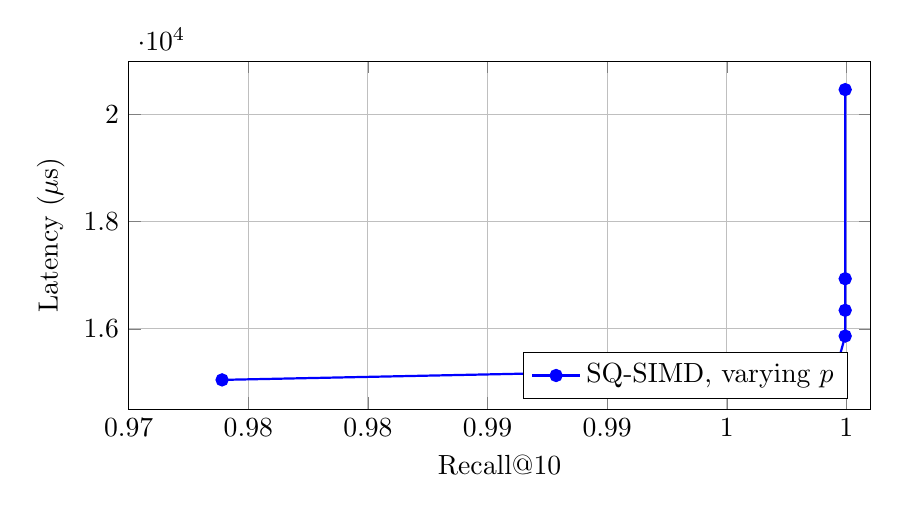
\begin{tikzpicture}
\begin{axis}[
    xlabel={Recall@10},
    ylabel={Latency ($\mu$s)},
    xmin=0.97, xmax=1.001,
    ymin=14500, ymax=21000,
    grid=major,
    width=11cm,
    height=6cm,
    legend pos=south east
]
\addplot[color=blue, mark=*, thick] coordinates {
    (0.973903,15045.7)
    (0.996800,15256.6)
    (0.999500,15136.8)
    (0.999950,15864.6)
    (0.999950,16346.0)
    (0.999950,16935.7)
    (0.999950,20469.2)
};
\addlegendentry{SQ-SIMD, varying $p$}
\end{axis}
\end{tikzpicture}
\caption{SQ-SIMD 的 Latency-Recall@10 Trade-off}
\label{fig:sq-tradeoff}
\end{figure}

PQ-SIMD 将 96 维向量拆分为多个子空间，并使用 ADC 查表估计距离。它的优势不是单条 FMA 更快，而是把距离计算转化为更短的查表累加，并大幅降低内存占用。fast 配置在 2988.9 $\mu$s 下达到 0.982952 的 recall，说明 PQ 对低延迟场景非常有效；若加入更充分的 rerank，则可以接近满 recall，但延迟回升到 5 ms 量级。这个结果体现了 PQ 的基本 trade-off：压缩越强，粗排越快，但需要用更大的候选集合或精排弥补量化误差。

\subsection{OpenMP / Pthread：共享内存多线程并行}

共享内存阶段的主要问题是如何把候选扫描任务分配给线程，并在每个线程维护局部 Top-$k$ 后高效归并。Pthread 与 OpenMP 都实现了 Flat、PQ、IVF、IVF-PQ 与 HNSW，其中 OpenMP 版本在多数代表性配置下更稳定，原因是线程池复用和循环调度开销更低。

\begin{table}[H]
\centering
\small
\caption{OpenMP / Pthread 代表性配置对比}
\label{tab:thread-main}
\begin{tabular}{llccc}
\toprule
算法 & 配置 & 版本 & Recall@10 & Latency ($\mu$s) \\
\midrule
Flat & 8 threads & Pthread & 0.999950 & 2040.90 \\
Flat & 8 threads & OpenMP & 0.999950 & 1470.77 \\
PQ & $M=16,p=1000,4T$ & OpenMP & 0.999950 & 1772.34 \\
IVF & nlist=256,nprobe=32,4T & Pthread & 0.990251 & 1290.95 \\
IVF & nlist=256,nprobe=32,4T & OpenMP & 0.990501 & 928.42 \\
HNSW & $M=32,ef=100,4T$ & OpenMP & 0.995601 & 178 \\
\bottomrule
\end{tabular}
\end{table}

\begin{breakablealgorithm}
\caption{共享内存候选扫描与局部 Top-$k$ 归并}
\label{alg:shared-topk}
\begin{algorithmic}[1]
\Require 候选集合 $C(q)$，查询向量 $q$，线程数 $T$，近邻数 $k$
\Ensure query 的 Top-$k$ 结果 $R$
\State 将 $C(q)$ 按连续区间或动态调度切分给 $T$ 个线程
\ForAll{线程 $t=0,1,\dots,T-1$ \textbf{in parallel}}
  \State 初始化线程局部最大堆 $H_t$，堆容量为 $k$
  \ForAll{候选向量 id $j$ 属于线程 $t$ 的任务区间}
    \State $s\gets \dist{x_j}{q}$
    \If{$H_t$ 未满 \textbf{or} $s$ 优于 $H_t$ 中最差元素}
      \State 将 $(s,j)$ 插入 $H_t$，必要时弹出最差元素
    \EndIf
  \EndFor
\EndFor
\State 将所有局部堆 $H_0,\dots,H_{T-1}$ 做 $T$ 路归并
\State \Return 全局最优的 $k$ 个候选作为 $R$
\end{algorithmic}
\end{breakablealgorithm}

该伪代码对应 Flat、PQ rerank、IVF list 内扫描等多个实现。区别在于 $C(q)$ 的来源不同：Flat 中 $C(q)$ 为全库；IVF 中为 nprobe 个倒排链表；PQ 中先由量化距离得到 Top-$p$，再对 $p$ 个候选精排。线程局部堆避免了每次距离计算都竞争全局堆，但最终归并仍会带来固定开销，因此当候选集合较小或线程过多时，加速比会下降。

线程数扩展实验进一步说明，共享内存并行存在明显的饱和点。以 Flat 全库扫描为例，OpenMP 与 Pthread 都能从 1 线程扩展到 8 线程，但继续增加到 16 线程后延迟反而回升，如表\ref{tab:thread-scaling}所示。这说明 DEEP100K 的 96 维内积在多线程下很快从计算瓶颈转向内存带宽、cache 争用与线程调度开销，单纯增加线程数并不能线性降低 latency。

\begin{table}[H]
\centering
\small
\caption{Flat 全库扫描的线程扩展表现}
\label{tab:thread-scaling}
\begin{tabular}{lccccc}
\toprule
版本 & 1T & 2T & 4T & 8T & 16T \\
\midrule
OpenMP latency ($\mu$s) & 4751.36 & 2790.79 & 1929.73 & 1470.77 & 1621.75 \\
Pthread latency ($\mu$s) & 6567.72 & 4050.93 & 2246.42 & 2040.90 & 2284.98 \\
\bottomrule
\end{tabular}
\end{table}

\begin{figure}[H]
\centering
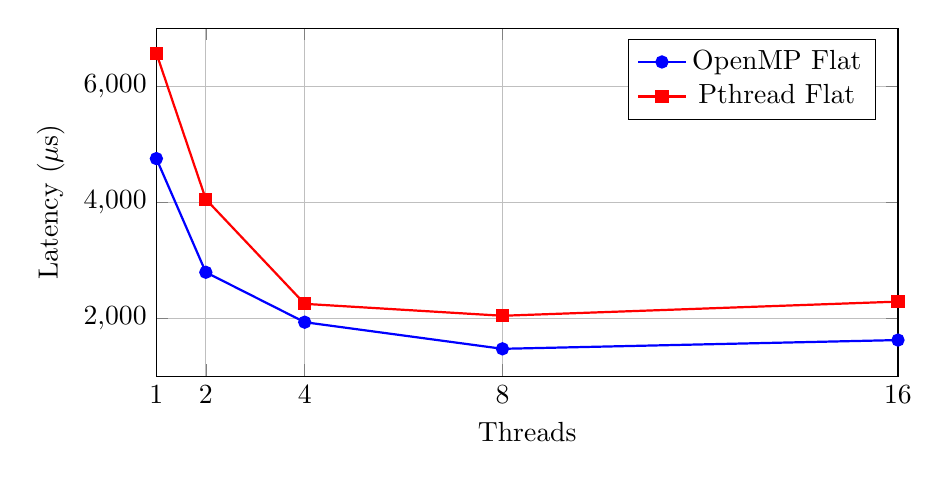
\begin{tikzpicture}
\begin{axis}[
    xlabel={Threads},
    ylabel={Latency ($\mu$s)},
    xtick={1,2,4,8,16},
    xmin=1, xmax=16,
    ymin=1000, ymax=7000,
    grid=major,
    width=11cm,
    height=6cm,
    legend pos=north east
]
\addplot[color=blue, mark=*, thick] coordinates {
    (1,4751.36) (2,2790.79) (4,1929.73) (8,1470.77) (16,1621.75)
};
\addlegendentry{OpenMP Flat}
\addplot[color=red, mark=square*, thick] coordinates {
    (1,6567.72) (2,4050.93) (4,2246.42) (8,2040.90) (16,2284.98)
};
\addlegendentry{Pthread Flat}
\end{axis}
\end{tikzpicture}
\caption{Flat 全库扫描的线程扩展曲线}
\label{fig:thread-scaling}
\end{figure}

从图\ref{fig:thread-scaling}看，OpenMP 在所有线程数下都优于 Pthread，且 1T 到 8T 的收益较稳定；16T 时两者均出现回退，说明此时主要限制已不是线程数量，而是内存系统和归并开销。该趋势也解释了为什么后续 IVF、PQ、HNSW 的代表性配置多选择 4T 或 8T，而不是盲目使用最高线程数。

IVF 是共享内存实验中最均衡的主方案。nprobe 控制被访问的倒排链表数量，直接决定候选规模。图\ref{fig:ivf-tradeoff}展示了 OpenMP IVF 在 nlist=100、4 线程下的 trade-off：nprobe 从 1 增至 32 时，Recall@10 从 0.636150 增至 0.997700，同时 latency 从 89.78 $\mu$s 上升到 1388.42 $\mu$s。

\begin{figure}[H]
\centering
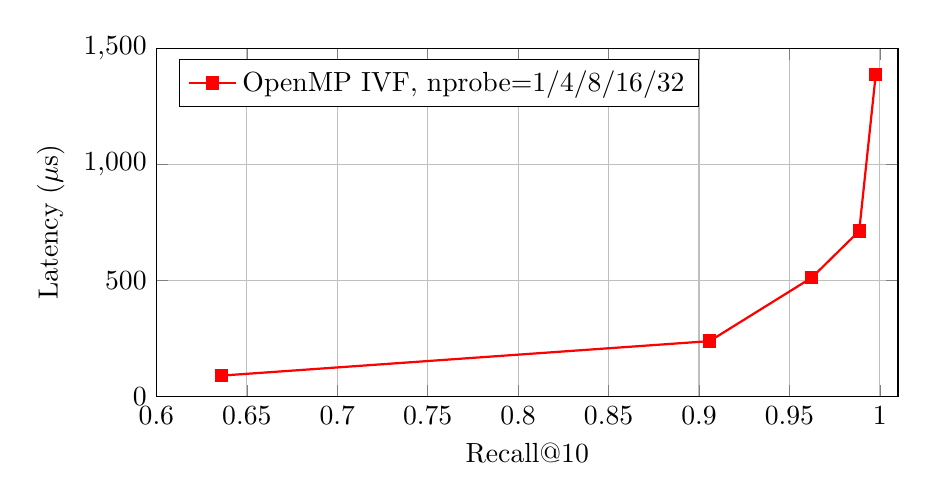
\begin{tikzpicture}
\begin{axis}[
    xlabel={Recall@10},
    ylabel={Latency ($\mu$s)},
    xmin=0.60, xmax=1.01,
    ymin=0, ymax=1500,
    grid=major,
    width=11cm,
    height=6cm,
    legend pos=north west
]
\addplot[color=red, mark=square*, thick] coordinates {
    (0.636150,89.78)
    (0.905853,238.36)
    (0.962302,511.91)
    (0.988551,713.08)
    (0.997700,1388.42)
};
\addlegendentry{OpenMP IVF, nprobe=1/4/8/16/32}
\end{axis}
\end{tikzpicture}
\caption{OpenMP IVF 的 Latency-Recall@10 Trade-off}
\label{fig:ivf-tradeoff}
\end{figure}

HNSW 则代表了另一类减少访问点数量的方法。它不依赖粗粒度聚类，而是在图上维护候选队列并逐步扩展邻居。ef 是查询阶段最关键的参数：ef 越大，搜索覆盖面越广，recall 越高，但访问节点也越多。图\ref{fig:hnsw-tradeoff}显示，OpenMP HNSW 在 $M=32$、4 线程下从 ef=10 到 ef=100，Recall@10 从 0.842354 提升到 0.995601，latency 从 45 $\mu$s 增至 178 $\mu$s。

\begin{figure}[H]
\centering
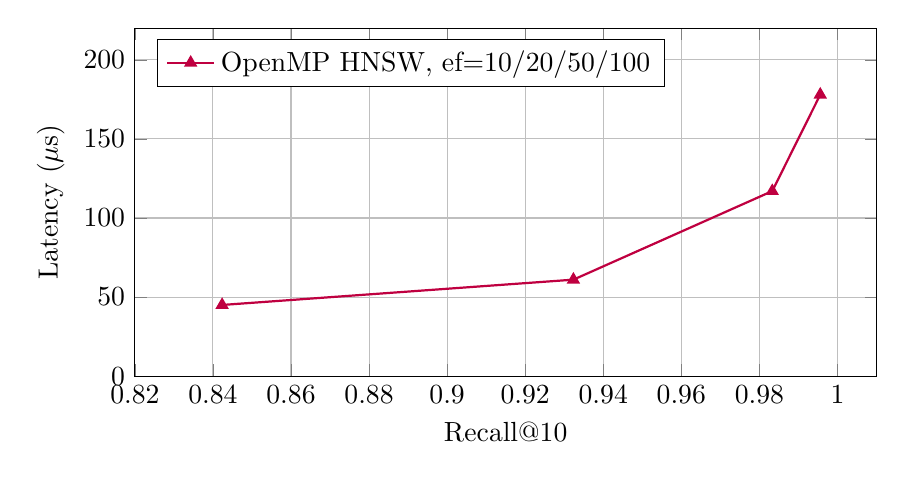
\begin{tikzpicture}
\begin{axis}[
    xlabel={Recall@10},
    ylabel={Latency ($\mu$s)},
    xmin=0.82, xmax=1.01,
    ymin=0, ymax=220,
    grid=major,
    width=11cm,
    height=6cm,
    legend pos=north west
]
\addplot[color=purple, mark=triangle*, thick] coordinates {
    (0.842354,45)
    (0.932354,61)
    (0.983302,117)
    (0.995601,178)
};
\addlegendentry{OpenMP HNSW, ef=10/20/50/100}
\end{axis}
\end{tikzpicture}
\caption{OpenMP HNSW 的 Latency-Recall@10 Trade-off}
\label{fig:hnsw-tradeoff}
\end{figure}

perf 计数器能解释为什么不同算法的加速形态差异很大。表\ref{tab:perf-counter}整理了平时实验中的代表性 perf 结果。串行 Flat 的指令量约 $71.47\times10^9$，SIMD Flat 降到约 $29.87\times10^9$，说明 SIMD 的主要收益来自减少指令数和提高单指令吞吐；OpenMP Flat 的 IPC 进一步提高到 1.0440，但 L1/LLC 命中率没有本质改变，因此最终仍受全库访存约束。IVF 与 HNSW 的关键不是让每次内积更快，而是减少被访问的候选点，使 cache 行为更集中。IVF-PQ 与 PQ 的 IPC 较高，但其查表和编码访问会引入更强的随机访存，因此 latency 未必随 IPC 单调下降。

\begin{table}[H]
\centering
\scriptsize
\caption{共享内存阶段 perf 计数器摘要}
\label{tab:perf-counter}
\begin{tabularx}{\textwidth}{lrrrrX}
\toprule
方案 & 指令数($10^9$) & CPI & IPC & L1 命中率 & 解释 \\
\midrule
Flat 串行 & 71.47 & 1.5868 & 0.6301 & 95.66\% & 指令多且全库访存，作为未优化基线 \\
SIMD Flat & 29.87 & 1.1412 & 0.8762 & 97.58\% & SIMD 降低指令数，distance 计算更紧凑 \\
OpenMP Flat & 30.48 & 0.9577 & 1.0440 & 97.78\% & 多线程提高吞吐，但访问规模不变 \\
OpenMP IVF & 42.58 & 0.6314 & 1.5836 & 99.59\% & 候选局部化后 cache 命中率更高 \\
OpenMP PQ & 82.81 & 0.5143 & 1.9443 & 99.75\% & 查表计算 IPC 高，但候选与表访问仍影响端到端 \\
OpenMP IVF-PQ & 103.87 & 0.4726 & 2.1156 & 99.78\% & 压缩索引带来高 IPC，同时 merge 与重排更复杂 \\
OpenMP HNSW & 0.054 & 0.5936 & 1.6844 & 97.19\% & 图搜索访问点少，查询阶段指令量最低 \\
\bottomrule
\end{tabularx}
\end{table}

这些 perf 结果也解释了第三节为什么不再重复基础 Flat/IVF/PQ/HNSW，而是把重点放在组合索引、数据布局和算子融合上。基础实验已经证明 SIMD 能降低距离计算指令量，OpenMP 能提升多 query 吞吐，IVF/HNSW/PQ 能减少或压缩候选；但当候选规模被压到两万级以后，新的瓶颈会转移到 PQ code 连续扫描、score 数组写回、top-$R$ 选择和 rerank 访存。因此后续进阶实验需要进一步观察同一候选集合下的数据重排、fused top-$R$ 和 query-level pipeline 是否能把 Latency-Recall 曲线整体左移。

\begin{figure}[H]
\centering
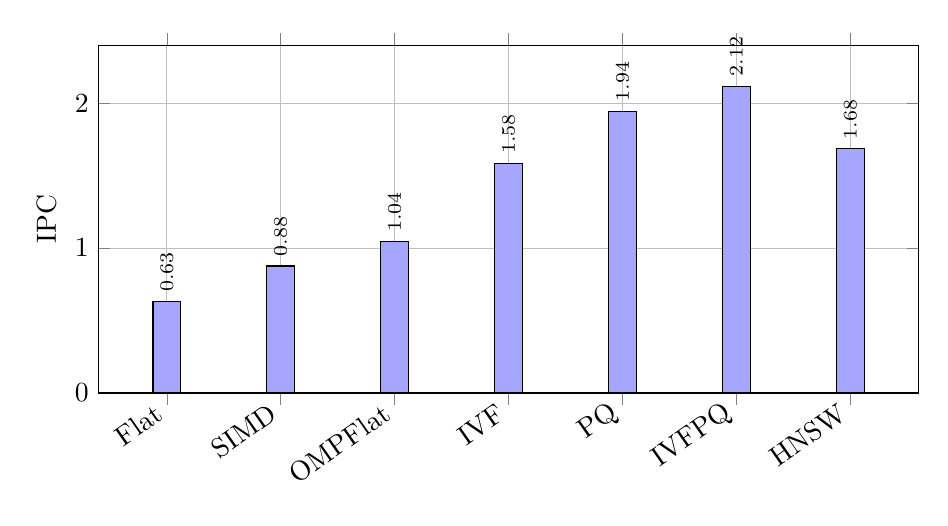
\begin{tikzpicture}
\begin{axis}[
    ybar,
    bar width=10pt,
    ylabel={IPC},
    symbolic x coords={Flat, SIMD, OMPFlat, IVF, PQ, IVFPQ, HNSW},
    xtick=data,
    xticklabel style={rotate=35, anchor=east},
    ymin=0, ymax=2.4,
    width=12cm,
    height=6cm,
    nodes near coords,
    nodes near coords style={font=\scriptsize, rotate=90, anchor=west},
    grid=major
]
\addplot[fill=blue!35] coordinates {
    (Flat,0.6301)
    (SIMD,0.8762)
    (OMPFlat,1.0440)
    (IVF,1.5836)
    (PQ,1.9443)
    (IVFPQ,2.1156)
    (HNSW,1.6844)
};
\end{axis}
\end{tikzpicture}
\caption{共享内存代表方案的 IPC 对比}
\label{fig:ipc-compare}
\end{figure}

图\ref{fig:ipc-compare}看似显示 PQ/IVF-PQ 的 IPC 最高，但这并不意味着它们端到端 latency 一定最低。IPC 衡量的是流水线利用率，而 ANNS 还包含候选生成、Top-$k$ 归并、随机访存和 rerank。HNSW 的 IPC 低于 IVF-PQ，但由于访问点数量少，最终查询延迟反而更低。这也是本文强调“机制分析必须和 Recall-Latency 曲线一起看”的原因。

IVF-PQ 是本阶段最能体现“压缩索引并不必然端到端最优”的方案。它同时使用 IVF 降低候选数量、PQ 降低候选打分成本，但在当前实现中还要承担码本查表、候选编号回映射、局部堆归并和必要精排的开销。原始 CSV 中可见，当 nlist=500、$M=16$、nprobe=50 时，OpenMP 4 线程达到 0.982403 recall、约 1687633 的原始计时值；Pthread 对同类配置可达到 0.991351 recall、约 2603086 的原始计时值。该结果说明 IVF-PQ 在内存压缩上有价值，但若目标是 DEEP100K 上的高 recall 低延迟，当前实验中 IVF 和 HNSW 的在线查询表现更稳定。

\begin{table}[H]
\centering
\scriptsize
\caption{IVF-PQ 原始记录中的代表性配置}
\label{tab:ivfpq-detail}
\begin{tabular}{lcccc}
\toprule
版本 & 配置 & 线程数 & Recall@10 & 原始计时字段 \\
\midrule
OpenMP IVF-PQ & nlist=500,$M=16$,nprobe=10 & 4T & 0.918052 & 884111 \\
OpenMP IVF-PQ & nlist=500,$M=16$,nprobe=50 & 4T & 0.982403 & 1687633 \\
Pthread IVF-PQ & nlist=100,$M=16$,nprobe=50 & 4T & 0.999300 & 4936890 \\
Pthread IVF-PQ & nlist=500,$M=16$,nprobe=50 & 4T & 0.991351 & 2603086 \\
\bottomrule
\end{tabular}
\end{table}

从算法机制看，Flat 的并行最直接，但仍需要访问全库；PQ 降低了单次候选打分的内存成本，但查表累加变成 memory-bound；IVF 通过 nprobe 明确控制候选规模，是本阶段最稳定的提交方案；HNSW 在查询阶段表现出更强的 recall-latency 优势，但构图成本更高，且基于 hnswlib 的实验更适合作为图索引参考配置。

\subsection{MPI：数据分片、通信与混合并行}

MPI 阶段将 base 数据按 rank 分片，每个进程维护局部索引；查询向量广播到所有 rank，各进程本地搜索得到局部 Top-$k$，最后由 rank0 汇总并 merge。该流程天然形成“进程间数据并行 + 进程内 OpenMP/Pthread 并行”的两级结构。

对原始 CSV 的整理显示，MPI 实验主要覆盖 blocking 通信、2 个 rank、MPI-IVF 与图索引分片两类路径，如表\ref{tab:mpi-audit}所示。因此本节重点分析“数据如何分片”和“rank 内是否继续使用 OpenMP/Pthread”，而不把 nonblocking 或 one-sided MPI 作为已验证结论。

\begin{table}[H]
\centering
\small
\caption{MPI 实验原始记录覆盖范围}
\label{tab:mpi-audit}
\begin{tabularx}{\textwidth}{lX}
\toprule
维度 & 覆盖情况 \\
\midrule
通信模式 & 原始记录均为 blocking，适合分析同步广播与汇总下的基线表现 \\
算法类型 & graph 记录 96 条，mpi\_ivf 记录 45 条，覆盖分片 HNSW、IVF+HNSW 与 MPI-IVF \\
rank 内线程模式 & OpenMP 66 条、Pthread 66 条、none 9 条，可比较混合并行收益 \\
比较限制 & 不足以评价非阻塞通信隐藏计算、动态负载均衡或跨 shard 图边维护 \\
\bottomrule
\end{tabularx}
\end{table}

\begin{breakablealgorithm}
\caption{MPI + OpenMP 两级并行查询}
\label{alg:mpi-query}
\begin{algorithmic}[1]
\Require rank $r$ 的局部索引 $\mathcal{I}_r$，查询集合 $Q$，近邻数 $k$
\Ensure rank0 上的全局 Top-$k$ 结果
\ForAll{$q_i\in Q$}
  \State rank0 读取 $q_i$，调用 \texttt{MPI\_Bcast} 广播到所有 rank
  \ForAll{rank $r=0,1,\dots,P-1$ \textbf{in parallel}}
    \State 在 $\mathcal{I}_r$ 上执行局部搜索；rank 内可继续使用 OpenMP/Pthread
    \State 得到局部结果 $R_{i,r}$，其中 id 已加上该 rank 的全局偏移
  \EndFor
  \State 各 rank 调用 \texttt{MPI\_Gather} 或点对点发送，将 $R_{i,r}$ 汇总到 rank0
  \State rank0 对 $P$ 个局部 Top-$k$ 做多路归并，得到全局 $R_i$
\EndFor
\end{algorithmic}
\end{breakablealgorithm}

算法\ref{alg:mpi-query}揭示了 MPI 阶段的两个不同瓶颈来源。对 IVF 来说，广播的 query 只有 96 个 float，回收的结果也只有 $P\times k$ 个二元组，通信量较小，局部搜索仍是主导；对 HNSW 来说，问题不在通信量，而在分片后图结构被切断，局部图搜索得到的候选不一定覆盖全局最优路径。

\begin{figure}[H]
\centering
\begin{tikzpicture}[node distance=0.75cm]
\node[flowstart] (rank0) {rank0\\读取 query};
\node[flowproc, below=of rank0] (bcast) {MPI\_Bcast\\广播 query};
\node[flowidx, below left=1.0cm and 2.8cm of bcast] (r0) {rank0 shard\\局部 IVF/HNSW\\OpenMP/Pthread};
\node[flowidx, below=1.0cm of bcast] (r1) {rank1 shard\\局部 IVF/HNSW\\OpenMP/Pthread};
\node[flowidx, below right=1.0cm and 2.8cm of bcast] (rn) {rank $P-1$ shard\\局部 IVF/HNSW\\OpenMP/Pthread};
\node[flowproc, below=2.4cm of bcast] (local) {各 rank 产生局部 Top-$k$};
\node[flowproc, below=of local] (gather) {MPI\_Gather / Send\\收集局部结果};
\node[floweval, below=of gather] (merge) {rank0 全局 Top-$k$ merge\\计算 Recall@10};
\draw[flowarrow] (rank0) -- (bcast);
\draw[flowarrow] (bcast) -- (r0);
\draw[flowarrow] (bcast) -- (r1);
\draw[flowarrow] (bcast) -- (rn);
\draw[flowarrow] (r0) |- (local);
\draw[flowarrow] (r1) -- (local);
\draw[flowarrow] (rn) |- (local);
\draw[flowarrow] (local) -- (gather);
\draw[flowarrow] (gather) -- (merge);
\end{tikzpicture}
\caption{MPI 两级并行查询流程}
\label{fig:mpi-flow}
\end{figure}

图\ref{fig:mpi-flow}对应本实验的 blocking 通信基线。由于每条 query 的广播数据量固定且较小，MPI-IVF 的主要优化空间在各 rank 的局部索引质量、局部候选规模和 rank 内线程并行；而分片 HNSW 的主要问题是全局图导航路径被分割，单纯增加 rank 数不一定能提升 recall。

\begin{table}[H]
\centering
\small
\caption{MPI-IVF 代表性配置（按报告解释换算为 $\mu$s/query）}
\label{tab:mpi-ivf}
\begin{tabular}{lcccc}
\toprule
算法 & 配置 & 线程模式 & Recall@10 & Latency ($\mu$s) \\
\midrule
MPI-IVF & nlist=32,nprobe=4,4T & OpenMP & 0.97 & 1267.935 \\
MPI-IVF & nlist=32,nprobe=8,4T & OpenMP & 1.00 & 1040.504 \\
MPI-IVF & nlist=32,nprobe=16,4T & OpenMP & 1.00 & 1212.402 \\
MPI-IVF & nlist=64,nprobe=16,4T & OpenMP & 1.00 & 1787.545 \\
MPI-IVF & nlist=128,nprobe=16,4T & OpenMP & 0.99 & 3685.551 \\
\bottomrule
\end{tabular}
\end{table}

MPI-IVF 的一个重要现象是：nlist 并不是越大越好。nlist 太小会使单个倒排链表过长，精排候选多；nlist 太大又会使分片后的每个 list 过稀，聚类质量和负载均衡变差。在当前分片规模下，nlist=32,nprobe=8 是最均衡的配置。

图\ref{fig:mpi-pareto}给出了 MPI 阶段三类算法的 Pareto 散点。MPI-IVF 在高 recall 区间最稳定；分片 HNSW 的延迟最低，但由于跨 shard 图边缺失，recall 上限约在 0.98 左右；IVF+HNSW 能体现图精排思路，但当前实现存在临时图或多层结构带来的额外开销。

\begin{figure}[H]
\centering
\begin{tikzpicture}
\begin{axis}[
    xlabel={Latency ($\mu$s, log scale)},
    ylabel={Recall@10},
    xmode=log,
    xmin=100, xmax=1e5,
    ymin=0.80, ymax=1.02,
    grid=both,
    width=11cm,
    height=6.5cm,
    legend pos=south west
]
\addplot[only marks, mark=*, mark size=2.4pt, color=blue] coordinates {
    (1267.935,0.97) (1040.504,1.00) (1212.402,1.00)
    (1889.236,0.96) (1856.796,0.99) (1787.545,1.00)
    (3048.411,0.91) (3521.582,0.97) (3685.551,0.99)
};
\addlegendentry{MPI-IVF}
\addplot[only marks, mark=triangle*, mark size=2.4pt, color=red] coordinates {
    (250,0.98) (324,0.98) (806,0.96) (19896,0.97) (32059,0.97)
};
\addlegendentry{分片 HNSW}
\addplot[only marks, mark=square*, mark size=2.4pt, color=green!60!black] coordinates {
    (522.474,0.86) (673.455,0.91) (1457.970,0.93)
    (2718.925,0.98) (3286.303,0.94)
};
\addlegendentry{IVF+HNSW}
\end{axis}
\end{tikzpicture}
\caption{MPI 阶段三类算法的 Recall-Latency 散点图}
\label{fig:mpi-pareto}
\end{figure}

MPI 结果说明，ANNS 的 MPI 化不能只关注通信 API 本身。对于 IVF，query 广播和 Top-$k$ 汇总消息很小，主要瓶颈仍是每个 rank 的局部 fine search；因此 rank 内 OpenMP 能带来显著收益。对于 HNSW，简单数据分片会切断全局导航路径，导致 recall 上限下降；要进一步提高图索引 MPI 性能，需要保留跨 shard 边或共享高质量入口点。

\subsection{GPU：Query Batch 与有效候选 Pair 压缩}

GPU 阶段的核心结论是：单条 query 很难充分利用 GPU，必须把多个 query 组成 batch。实验实现了三类方案：Flat Batch 矩阵 baseline、IVF Cluster-Union baseline、IVF Compact Pair Optimization。代表性结果如表\ref{tab:gpu-main}所示。

\begin{table}[H]
\centering
\small
\caption{GPU 阶段代表性结果}
\label{tab:gpu-main}
\begin{tabular}{lcccc}
\toprule
算法 & 配置 & Recall@10 & Latency ($\mu$s) & 平均候选数 \\
\midrule
GPU Flat Batch & batch=128, 精确全量 & 0.999950 & 375.686 & 100000.0 \\
GPU IVF Union & nlist=64,nprobe=8 & 0.968000 & 377.067 & 16218.9 \\
GPU IVF Compact & nlist=64,nprobe=8 & 0.968000 & 96.130 & 16218.9 \\
GPU IVF Compact & nlist=64,nprobe=16 & 0.991550 & 180.781 & 29141.9 \\
\bottomrule
\end{tabular}
\end{table}

Flat Batch 是精确 baseline，它为每个 $(query,base)$ pair 启动距离计算，召回率接近 1，但需要生成完整 $m\times N$ 距离矩阵并回传 CPU。IVF Union 保留簇矩阵乘法形式，但 batch 内不同 query 的最近簇不一致，导致簇并集内存在大量无效计算。IVF Compact 则只展开实际需要访问的 $(query,candidate)$ pair，从而避免无效簇计算。

\begin{breakablealgorithm}
\caption{GPU IVF Compact 有效 Pair 搜索}
\label{alg:gpu-compact}
\begin{algorithmic}[1]
\Require batch 查询 $B$，centroid 数组，倒排链表 offsets，近邻数 $k$
\Ensure batch 内每条 query 的 Top-$k$ 结果
\State 在 GPU 上计算 batch 内 query 到所有 centroid 的距离
\State 对每条 query 选择最近的 nprobe 个 centroid
\State 根据各 query 的 nprobe 个 list 计算有效 pair 总数与 prefix-sum offset
\State 构造紧凑 pair 数组 $P=\{(query\_id,base\_id)\}$，只包含实际需要访问的候选
\State 启动 \texttt{indexed\_score\_kernel}，对 $P$ 中每个 pair 计算距离
\State 将紧凑距离结果回传 CPU，按 query 分段执行 Top-$k$ 选择
\State \Return batch 内所有 query 的 Top-$k$
\end{algorithmic}
\end{breakablealgorithm}

Compact 与 Union 的根本区别在算法\ref{alg:gpu-compact}第 3-4 行。Union 为了保留矩阵计算形式，会把 batch 中不同 query 的候选簇取并集，导致某些 query 计算了并不需要的簇；Compact 则先显式展开有效 pair，再只对这些 pair 打分。前者牺牲计算量换规整矩阵，后者牺牲部分访存规整性换更少的距离项和更少的 D2H 回传。

\begin{figure}[H]
\centering
\begin{tikzpicture}[node distance=0.75cm]
\node[flowstart] (batch) {Query batch};
\node[flowproc, below=of batch] (centroid) {计算 query-centroid 距离\\选择 nprobe 个簇};
\node[flowidx, below left=1.0cm and 2.2cm of centroid] (union) {Union 路径\\batch 簇并集};
\node[flowidx, below right=1.0cm and 2.2cm of centroid] (compact) {Compact 路径\\按 query 展开有效 pair};
\node[flowproc, below=of union] (unionkernel) {对簇并集做矩阵式打分\\包含无效 pair};
\node[flowproc, below=of compact] (compactkernel) {indexed kernel 打分\\仅计算有效 pair};
\node[flowproc, below=2.6cm of centroid] (d2h) {D2H 回传距离结果};
\node[floweval, below=of d2h] (topk) {CPU 分 query Top-$k$\\统计 recall/latency};
\draw[flowarrow] (batch) -- (centroid);
\draw[flowarrow] (centroid) -- (union);
\draw[flowarrow] (centroid) -- (compact);
\draw[flowarrow] (union) -- (unionkernel);
\draw[flowarrow] (compact) -- (compactkernel);
\draw[flowarrow] (unionkernel) |- (d2h);
\draw[flowarrow] (compactkernel) |- (d2h);
\draw[flowarrow] (d2h) -- (topk);
\end{tikzpicture}
\caption{GPU IVF Union 与 Compact 的执行流程对比}
\label{fig:gpu-union-compact-flow}
\end{figure}

图\ref{fig:gpu-union-compact-flow}与 profiling 结果相互印证：Union 的矩阵形态并没有转化为端到端优势，因为簇并集会扩大实际打分和回传规模；Compact 虽然 indexed 访问更不规则，但能从源头减少 pair 数，使 kernel 总时间和 D2H 压力同时下降。

\begin{figure}[H]
\centering
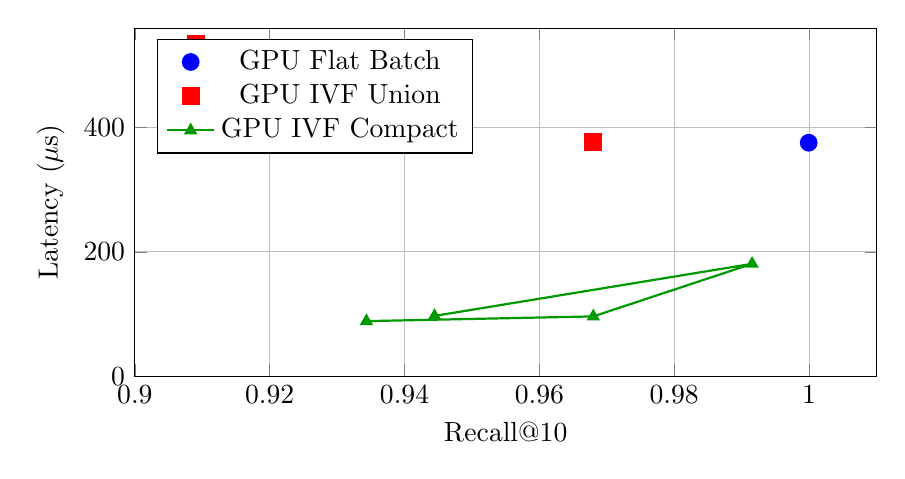
\begin{tikzpicture}
\begin{axis}[
    xlabel={Recall@10},
    ylabel={Latency ($\mu$s)},
    xmin=0.90, xmax=1.01,
    ymin=0, ymax=560,
    grid=major,
    width=11cm,
    height=6cm,
    legend pos=north west
]
\addplot[only marks, mark=*, mark size=3pt, color=blue] coordinates {
    (0.999950,375.686)
};
\addlegendentry{GPU Flat Batch}
\addplot[only marks, mark=square*, mark size=3pt, color=red] coordinates {
    (0.909100,534.651) (0.968000,377.067) (0.944450,397.801)
};
\addlegendentry{GPU IVF Union}
\addplot[color=green!60!black, mark=triangle*, thick] coordinates {
    (0.934350,88.520)
    (0.968000,96.130)
    (0.991550,180.781)
    (0.944450,96.915)
};
\addlegendentry{GPU IVF Compact}
\end{axis}
\end{tikzpicture}
\caption{GPU 阶段 Latency-Recall@10 Trade-off}
\label{fig:gpu-tradeoff}
\end{figure}

以 nlist=64,nprobe=8 为例，IVF Union 与 IVF Compact 的 Recall@10 都是 0.968000，但延迟分别为 377.067 $\mu$s 与 96.130 $\mu$s，Compact 约快 $3.92\times$。profiling 结果也验证了这一点：Flat 的核心 kernel 总时间约 411.290 ms，Union 的 cluster kernel 总时间约 329.498 ms 且 launch 次数高达 6364 次，而 Compact 的 indexed kernel 总时间仅约 54.446 ms。Compact 的单个 pair 访存并不如矩阵乘法规整，但它减少了实际距离项和 D2H 回传规模，因此端到端更优。

\begin{table}[H]
\centering
\scriptsize
\caption{GPU profiling 中的 kernel 摘要}
\label{tab:gpu-kernel-profile}
\begin{tabular}{lrrrrr}
\toprule
Kernel & 总时间(ms) & 调用次数 & 平均时间($\mu$s) & Memory Throughput & SM Throughput \\
\midrule
flat\_score\_kernel & 411.290 & 32 & 12852.812 & 97.64\% & 12.03\% \\
cluster\_score\_kernel & 329.498 & 6364 & 51.775 & 92.49\% & 11.47\% \\
indexed\_score\_kernel & 54.446 & 63 & 864.226 & 85.67\% & 10.67\% \\
\bottomrule
\end{tabular}
\end{table}

\begin{figure}[H]
\centering
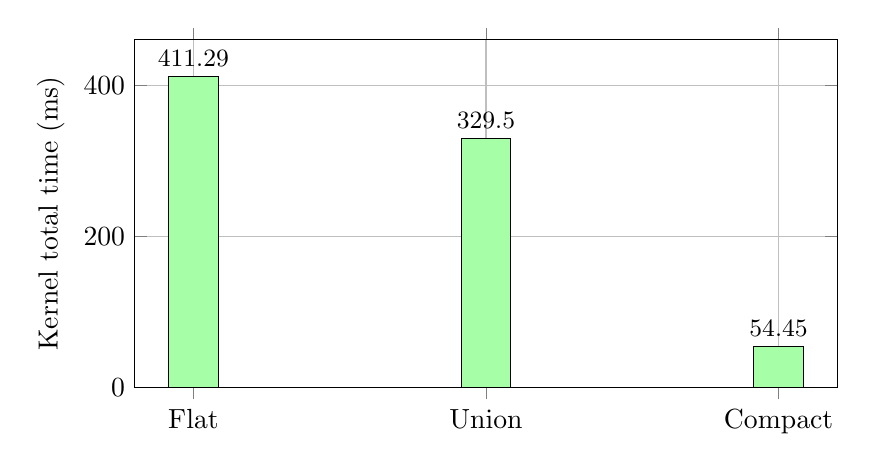
\begin{tikzpicture}
\begin{axis}[
    ybar,
    bar width=18pt,
    ylabel={Kernel total time (ms)},
    symbolic x coords={Flat, Union, Compact},
    xtick=data,
    ymin=0, ymax=460,
    width=10.5cm,
    height=6cm,
    nodes near coords,
    nodes near coords style={font=\small},
    grid=major
]
\addplot[fill=green!35] coordinates {
    (Flat,411.290)
    (Union,329.498)
    (Compact,54.446)
};
\end{axis}
\end{tikzpicture}
\caption{GPU 三类 kernel 总时间对比}
\label{fig:gpu-kernel-time}
\end{figure}

表\ref{tab:gpu-kernel-profile}说明三类 GPU 方案的瓶颈都更接近 memory-bound，而不是 SM 算力耗尽。Flat kernel 的显存吞吐占比最高，是因为它规整地遍历完整 base；但它必须处理 $batch\times N$ 的全部 pair。Union 的单次 kernel 很短，却因为簇并集和批内不一致导致调用次数过多。Compact 的 indexed kernel 不是最规整的访存模式，但它把 kernel 总时间压到 54.446 ms，说明减少无效 pair 比保持矩阵形态更重要。

\begin{table}[H]
\centering
\small
\caption{GPU profiling 中的主机-设备传输摘要}
\label{tab:gpu-memcpy-profile}
\begin{tabular}{lrrrr}
\toprule
方向 & 总时间(ms) & 调用次数 & 总传输量(MB) & 平均传输量(MB) \\
\midrule
D2H & 191.015 & 6459 & 1637.693 & 0.254 \\
H2D & 41.032 & 6711 & 344.452 & 0.051 \\
\bottomrule
\end{tabular}
\end{table}

D2H 总时间明显高于 H2D，说明 GPU ANN 不能只优化距离计算 kernel，还必须减少需要回传 CPU 的中间结果规模。这与代码中的设计一致：Flat Batch 回传完整距离矩阵，Union 回传簇并集结果，Compact 只回传有效 pair 的距离或压缩候选结果，因此在端到端 latency 上优势更明显。

\subsection{横向融合分析}

表\ref{tab:global-main}汇总了各阶段最具代表性的配置。该表不用于跨硬件绝对排名，而用于说明不同并行环境和索引算法的主要优势与瓶颈。

\begin{table}[H]
\centering
\scriptsize
\caption{不同并行环境与算法的代表性对比}
\label{tab:global-main}
\begin{tabularx}{\textwidth}{llccX}
\toprule
并行环境 & 代表算法 / 配置 & Recall@10 & Latency ($\mu$s) & 主要瓶颈与适用场景 \\
\midrule
SIMD & Flat-SIMD, NEON & 0.999950 & 7073.44 & 不改变候选集合，适合作为精确 CPU 距离计算基线；受内存带宽限制 \\
SIMD & PQ-SIMD rerank & 0.999950 & 5026.63 & 量化压缩降低访存，需通过 rerank 保证高 recall \\
OpenMP & IVF, nlist=256,nprobe=32,4T & 0.990501 & 928.42 & 访问点数量显著下降，是共享内存阶段最稳定方案 \\
OpenMP & HNSW, $M=32,ef=100,4T$ & 0.995601 & 178 & 查询延迟低，构图成本较高，适合大量重复查询 \\
MPI & MPI-IVF, nlist=32,nprobe=8,OpenMP 4T & 1.000000 & 1040.504 & 数据分片 + rank 内 OpenMP，通信量小，局部 fine search 主导 \\
GPU & Flat Batch, batch=128 & 0.999950 & 375.686 & 精确 batch baseline，瓶颈在完整距离矩阵与 D2H 回传 \\
GPU & IVF Compact, nlist=64,nprobe=16 & 0.991550 & 180.781 & 有效 pair 压缩，兼顾较高 recall 与低延迟 \\
\bottomrule
\end{tabularx}
\end{table}

图\ref{fig:fused-pareto}把代表性方案放到同一张机制视角的 Pareto 图中。由于硬件环境不同，该图不用于绝对排名，而用于观察“减少候选规模”“压缩距离计算”“扩大并行粒度”三类优化在 recall-latency 平面上的相对位置。

\begin{figure}[H]
\centering
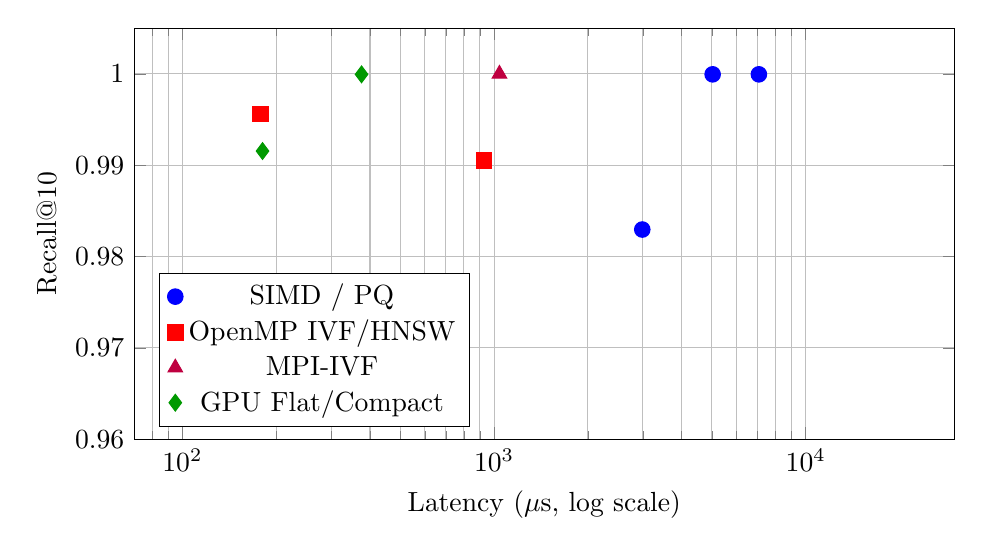
\begin{tikzpicture}
\begin{axis}[
    xlabel={Latency ($\mu$s, log scale)},
    ylabel={Recall@10},
    xmode=log,
    xmin=70, xmax=30000,
    ymin=0.96, ymax=1.005,
    grid=both,
    width=12cm,
    height=6.8cm,
    legend pos=south west
]
\addplot[only marks, mark=*, mark size=2.8pt, color=blue] coordinates {
    (7073.44,0.999950) (5026.63,0.999950) (2988.90,0.982952)
};
\addlegendentry{SIMD / PQ}
\addplot[only marks, mark=square*, mark size=2.8pt, color=red] coordinates {
    (928.42,0.990501) (178,0.995601)
};
\addlegendentry{OpenMP IVF/HNSW}
\addplot[only marks, mark=triangle*, mark size=3pt, color=purple] coordinates {
    (1040.504,1.000000)
};
\addlegendentry{MPI-IVF}
\addplot[only marks, mark=diamond*, mark size=3pt, color=green!60!black] coordinates {
    (375.686,0.999950) (96.130,0.968000) (180.781,0.991550)
};
\addlegendentry{GPU Flat/Compact}
\end{axis}
\end{tikzpicture}
\caption{代表性方案的融合 Latency-Recall@10 视图}
\label{fig:fused-pareto}
\end{figure}

图\ref{fig:fused-pareto}可以看出，Flat-SIMD 与 PQ rerank 都能保持接近精确的 recall，但 CPU 侧如果不减少候选数量，延迟仍在毫秒级；OpenMP IVF/HNSW 通过减少访问点进入更低延迟区域；GPU Flat Batch 说明强并行硬件可以把精确扫描压到数百微秒，但 D2H 与完整矩阵仍是限制；GPU Compact 则进一步把“候选减少”和“batch 并行”叠加起来，在 0.99 左右 recall 下得到更有竞争力的点。

如果从实际系统选型出发，Latency-Recall@10 trade-off 不能只看全局最低延迟，而要先确定业务可接受的 recall 下限。表\ref{tab:target-selection}按目标 recall 给出更细的选择逻辑。该表仍遵循同环境内比较优先的原则，但可以看出不同实验阶段的结果在系统层面如何互补。

\begin{table}[H]
\centering
\scriptsize
\caption{按目标 Recall@10 划分的关键方案选择}
\label{tab:target-selection}
\begin{tabularx}{\textwidth}{>{\raggedright\arraybackslash}p{2.3cm}>{\raggedright\arraybackslash}p{3.2cm}ccX}
\toprule
目标区间 & 优先考虑方案 & Recall@10 & Latency($\mu$s) & 选择理由 \\
\midrule
低延迟探索，Recall $\ge 0.90$ & GPU IVF Compact, nlist=64,nprobe=4 & 0.934350 & 88.520 & 有效 pair 数最少，适合对延迟极敏感且可接受近似误差的场景 \\
中高 recall，Recall $\ge 0.96$ & GPU IVF Compact, nlist=64,nprobe=8 & 0.968000 & 96.130 & 与 Union 同 recall，但约快 $3.92\times$，说明 pair 压缩有效 \\
高 recall，Recall $\ge 0.99$ & GPU IVF Compact, nlist=64,nprobe=16 & 0.991550 & 180.781 & 在较高 recall 下仍保持低于 0.2 ms 的端到端延迟 \\
高 recall CPU 查询 & OpenMP HNSW, $M=32,ef=100,4T$ & 0.995601 & 178 & 查询访问点极少，适合索引构建后反复查询 \\
稳定共享内存方案 & OpenMP IVF, nlist=256,nprobe=32,4T & 0.990501 & 928.42 & 参数含义清晰、实现稳定，便于控制 recall-latency 曲线 \\
接近精确结果 & GPU Flat Batch, batch=128 & 0.999950 & 375.686 & 精确全库扫描的 GPU batch baseline，代价是完整距离矩阵与 D2H 回传 \\
CPU 精确基线 & Flat-SIMD, NEON & 0.999950 & 7073.44 & 不改变结果集合，适合作为 CPU 精确距离计算优化基线 \\
\bottomrule
\end{tabularx}
\end{table}

为了把不同实验阶段真正融合起来，表\ref{tab:mechanism-matrix}从候选生成、距离计算、并行粒度、召回控制和风险五个维度对关键方案进行统一比较。

\begin{table}[H]
\centering
\scriptsize
\caption{关键方案的机制对比矩阵}
\label{tab:mechanism-matrix}
\begin{tabularx}{\textwidth}{lXXXXX}
\toprule
方案 & 候选生成 & 距离计算 & 并行粒度 & 召回控制 & 主要风险 \\
\midrule
Flat-SIMD & 全库候选，无近似剪枝 & NEON 向量化内积 & 向量维度内并行 & 不损失 recall & 候选规模固定为 $N$，受带宽限制 \\
PQ / SQ & 量化距离粗排 Top-$p$ & 查表或 uint8 累加后 rerank & 候选打分并行 & $p$ 越大 recall 越高 & 量化误差与查表随机访存 \\
OpenMP IVF & nprobe 个倒排链表 & list 内原始向量精排 & 线程级候选扫描 & nprobe 控制曲线 & nlist/nprobe 不匹配会负载不均 \\
OpenMP HNSW & 图搜索动态扩展候选 & 访问节点的精确距离 & 邻居扩展与 query 并行 & ef 控制搜索宽度 & 构图成本高，分片后图路径易断 \\
MPI-IVF & rank 内局部 IVF 候选 & 每个 rank 局部精排 & 进程分片 + 线程并行 & nlist/nprobe 与 rank 数共同影响 & 通信虽小但全局负载均衡困难 \\
GPU Compact & 每条 query 的有效 pair & indexed kernel 打分 & batch pair 并行 & nprobe 控制候选规模 & 访存不如矩阵规整，Top-$k$ 仍在 CPU \\
\bottomrule
\end{tabularx}
\end{table}

该矩阵体现了一个重要结论：同一种算法在不同并行环境下的瓶颈可能完全不同。例如 IVF 在 OpenMP 中主要考虑线程调度和 list 负载均衡，在 MPI 中还要考虑 rank 分片后的局部候选覆盖，在 GPU 中则要考虑 list 展开后是否产生大量无效 pair。因此报告中的“并行方案对比”不是简单比较 SIMD、OpenMP、MPI、GPU 四个标签，而是比较算法结构与硬件并行粒度是否匹配。

从全学期实验可以归纳出四条融合主线。

\begin{enumerate}
  \item \textbf{只优化距离计算不足以解决 ANNS 问题。} Flat-SIMD 能获得约 3 倍加速，并且不损失 recall，但仍需访问全部 100000 条 base 向量，因此它更像精确距离计算基线。真正的低延迟来自减少访问点数量，如 IVF 用 nprobe 控制倒排链表数量、HNSW 用 ef 控制图搜索宽度、GPU Compact 只展开有效 $(query,candidate)$ pair。
  \item \textbf{索引参数本质上是在移动 Pareto 曲线。} SQ 的 $p$、PQ 的粗排候选数、IVF 的 nlist/nprobe、HNSW 的 ef 都会改变候选集合大小。参数过小会丢失真实近邻，参数过大又会退化为接近全库扫描。实验中 SQ 在 $p=500$ 后 recall 基本饱和，IVF 在 nprobe 提高时延迟近似随候选规模增长，HNSW 则用较少访问点获得更高 recall，是图索引在在线查询阶段的主要优势。
  \item \textbf{量化和索引会把瓶颈从 compute-bound 转移到 memory-bound。} SQ/PQ 降低了存储和乘加开销，但查表累加、候选堆维护、随机访存会成为新瓶颈。perf 计数器中 PQ/IVF-PQ 的 IPC 很高，却不必然对应最低 latency，说明端到端性能还受候选归并和内存访问模式影响。多线程也不是越多越好，Flat 在 8 线程后出现回升，体现了带宽与调度饱和。
  \item \textbf{并行环境决定了最有效的任务划分粒度。} SIMD 适合向量维度内并行，OpenMP/Pthread 适合候选集合并行，MPI 适合 base 分片并行，GPU 适合 query batch 与大规模 pair 并行。若任务划分粒度与硬件不匹配，就会出现负优化，例如 MPI 图索引的跨 shard 导航丢失、GPU Union 的簇并集无效计算、Pthread 线程管理开销过大等。
\end{enumerate}

因此，较完整的 ANNS 系统不应只选择单一优化技术，而应组合使用：底层距离计算使用 SIMD 或 GPU kernel，候选生成使用 IVF/HNSW 减少访问点，候选集合内部使用 OpenMP/MPI/GPU 做并行扫描，最后用 rerank 或更大的 ef/nprobe/p 在目标 recall 下调节 latency。对 DEEP100K，本学期实验中最清晰的工程路线是：CPU 侧用 OpenMP IVF 作为稳定可解释方案，用 HNSW 作为高查询量场景的低延迟图索引方案；GPU 侧优先使用 Compact 而不是 Union，因为减少无效 pair 和 D2H 结果规模比保留矩阵形态更重要。

\section{算法集成与进阶}

\subsection{算法设计与实验方案}


\begin{table}[H]
\centering
\scriptsize
\caption{进阶实验方案与新增机制}
\label{tab:advanced-schemes}
\setlength{\tabcolsep}{4pt}
\renewcommand{\arraystretch}{1.12}
\begin{tabularx}{\textwidth}{>{\raggedright\arraybackslash}p{0.28\textwidth}>{\raggedright\arraybackslash}p{0.19\textwidth}>{\raggedright\arraybackslash}p{0.21\textwidth}>{\raggedright\arraybackslash}X}
\toprule
方案 & 索引组合 & 新增机制 & 主要验证点  \\
\midrule
Residual-IVF-PQ-Rerank & IVF + residual PQ + exact rerank & 残差编码替代原向量粗排 & 验证压缩打分与 rerank 闭环 \\
OPQ-IVF-PQ-Rerank & IVF + OPQ-lite + PQ + rerank & 按 residual 方差重排维度 & 均衡子空间方差，观察量化误差变化 \\
IVF-HNSW-OPQ-PQ-Rerank & IVF + centroid graph + OPQ/PQ & 图路由替代完整 centroid 扫描 & 减少 coarse routing 访问点并检查 recall 稳定性 \\
Reordered-IVF-HNSW-OPQ-PQ & 上述组合 & list 内 ID/code/vector 连续化 & 验证顺序访存与 cache locality \\
Fused-Reordered-IVF-HNSW-OPQ-PQ & 上述组合 & PQ 查表累加与 top-$R$ 融合 & 减少 score 写回、排序和中间结果 \\
Pipeline-OMP-SIMD 版本 & 上述最终方案 & query 级 OpenMP + AVX2 rerank & 结合 24 线程 CPU 观察批量吞吐 \\
\bottomrule
\end{tabularx}
\end{table}


\begin{table}[H]
\centering
\scriptsize
\caption{实验规划}
\label{tab:advanced-plan}
\setlength{\tabcolsep}{4pt}
\renewcommand{\arraystretch}{1.12}
\begin{tabularx}{\textwidth}{>{\raggedright\arraybackslash}p{0.17\textwidth}>{\raggedright\arraybackslash}p{0.27\textwidth}>{\raggedright\arraybackslash}p{0.27\textwidth}>{\raggedright\arraybackslash}X}
\toprule
实验组 & 方案设置 & 控制变量 / 扫描变量 & Profiling 关注点 \\
\midrule
A：残差压缩集成 & Residual-IVF-PQ-Rerank；np8/16/24/32，R200/500/800/1000 & 扫描 $nprobe$、$R$；覆盖低延迟、中高 recall、高 recall 区间 & PQ 扫描、显式 top-$R$、rerank 比例 \\
B：OPQ 量化优化 & OPQ-IVF-PQ-Rerank；与 A 使用同一组参数 & 相同候选规模下加入 OPQ-lite 维度重排 & recall 增益与 permutation 访存代价 \\
C：IVF-HNSW 融合 & IVF-HNSW-OPQ-PQ-Rerank；ef16/32/48/64 & 固定 $nprobe=16,R=500$；只改变 graph 搜索宽度 & centroid 访问数、图扩展成本、coarse 漏召回 \\
D：重排与融合 & Reordered / Fused-Reordered；np8/16/24 & 候选集基本不变；对比 list 布局与 fused top-$R$ & 顺序访存、score 写回、nth-element 开销 \\
E：硬件协同执行 & Pipeline-OMP-SIMD；np8/16/24 & 索引结构不变；开启 query-level OpenMP 与 AVX2 rerank & wall-time latency、吞吐与并行阶段重叠 \\
\bottomrule
\end{tabularx}
\end{table}

图\ref{fig:advanced-scheme-flows}按 A-E 分别给出了本节五组方案的查询或构建流程。可以看到，A 和 B 的主要差异在 PQ 编码空间，C 的差异在 coarse centroid 的选择方式，D 的差异在候选表布局与 top-$R$ 算子，E 的差异则在执行层把多条 query 组织为 OpenMP pipeline。

\begin{figure}[H]
\centering
\scriptsize
\resizebox{\textwidth}{!}{
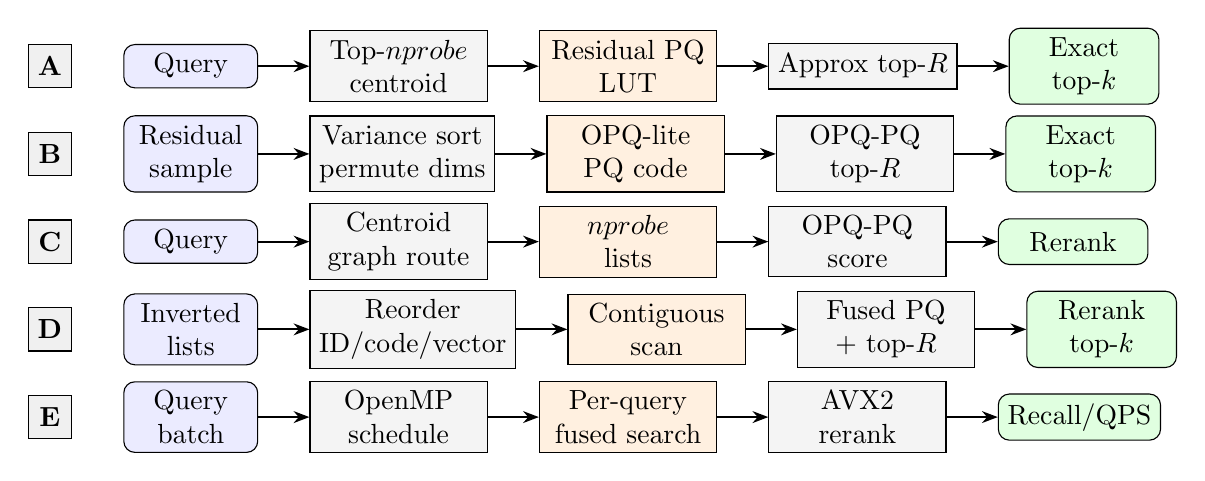
\begin{tikzpicture}[node distance=0.55cm and 0.65cm]
\tikzset{
  astart/.style={rectangle, rounded corners, draw=black, fill=blue!8, align=center, minimum width=1.7cm, minimum height=0.55cm},
  aproc/.style={rectangle, draw=black, fill=gray!9, align=center, minimum width=2.25cm, minimum height=0.58cm},
  aidx/.style={rectangle, draw=black, fill=orange!12, align=center, minimum width=2.25cm, minimum height=0.58cm},
  aend/.style={rectangle, rounded corners, draw=black, fill=green!12, align=center, minimum width=1.9cm, minimum height=0.58cm},
  alabel/.style={rectangle, draw=black, fill=black!6, align=center, minimum width=0.55cm, minimum height=0.55cm, font=\bfseries}
}

\node[alabel] (la) {A};
\node[astart, right=of la] (a1) {Query};
\node[aproc, right=of a1] (a2) {Top-$nprobe$\\centroid};
\node[aidx, right=of a2] (a3) {Residual PQ\\LUT};
\node[aproc, right=of a3] (a4) {Approx top-$R$};
\node[aend, right=of a4] (a5) {Exact\\top-$k$};
\draw[flowarrow] (a1) -- (a2);
\draw[flowarrow] (a2) -- (a3);
\draw[flowarrow] (a3) -- (a4);
\draw[flowarrow] (a4) -- (a5);

\node[alabel, below=of la] (lb) {B};
\node[astart, right=of lb] (b1) {Residual\\sample};
\node[aproc, right=of b1] (b2) {Variance sort\\permute dims};
\node[aidx, right=of b2] (b3) {OPQ-lite\\PQ code};
\node[aproc, right=of b3] (b4) {OPQ-PQ\\top-$R$};
\node[aend, right=of b4] (b5) {Exact\\top-$k$};
\draw[flowarrow] (b1) -- (b2);
\draw[flowarrow] (b2) -- (b3);
\draw[flowarrow] (b3) -- (b4);
\draw[flowarrow] (b4) -- (b5);

\node[alabel, below=of lb] (lc) {C};
\node[astart, right=of lc] (c1) {Query};
\node[aproc, right=of c1] (c2) {Centroid\\graph route};
\node[aidx, right=of c2] (c3) {$nprobe$\\lists};
\node[aproc, right=of c3] (c4) {OPQ-PQ\\score};
\node[aend, right=of c4] (c5) {Rerank};
\draw[flowarrow] (c1) -- (c2);
\draw[flowarrow] (c2) -- (c3);
\draw[flowarrow] (c3) -- (c4);
\draw[flowarrow] (c4) -- (c5);

\node[alabel, below=of lc] (ld) {D};
\node[astart, right=of ld] (d1) {Inverted\\lists};
\node[aproc, right=of d1] (d2) {Reorder\\ID/code/vector};
\node[aidx, right=of d2] (d3) {Contiguous\\scan};
\node[aproc, right=of d3] (d4) {Fused PQ\\+ top-$R$};
\node[aend, right=of d4] (d5) {Rerank\\top-$k$};
\draw[flowarrow] (d1) -- (d2);
\draw[flowarrow] (d2) -- (d3);
\draw[flowarrow] (d3) -- (d4);
\draw[flowarrow] (d4) -- (d5);

\node[alabel, below=of ld] (le) {E};
\node[astart, right=of le] (e1) {Query\\batch};
\node[aproc, right=of e1] (e2) {OpenMP\\schedule};
\node[aidx, right=of e2] (e3) {Per-query\\fused search};
\node[aproc, right=of e3] (e4) {AVX2\\rerank};
\node[aend, right=of e4] (e5) {Recall/QPS};
\draw[flowarrow] (e1) -- (e2);
\draw[flowarrow] (e2) -- (e3);
\draw[flowarrow] (e3) -- (e4);
\draw[flowarrow] (e4) -- (e5);
\end{tikzpicture}}
\caption{五组进阶方案的流程图总览}
\label{fig:advanced-scheme-flows}
\end{figure}

\subsubsection{方案 A：Residual-IVF-PQ-Rerank}

方案 A 是本节的组合起点。其原理是先用 IVF coarse centroid 将全库划分为多个倒排桶，查询时只访问与 $q$ 最近的 $nprobe$ 个桶；桶内不直接对全部候选做精确内积，而是使用残差 PQ 编码近似估计候选得分。残差形式为 $r_x=x-c(x)$，查询在某个倒排桶 $l$ 中对应的残差查询为 $q-c_l$。这样 PQ 查表估计的是 query 与 residual codeword 的相似度，再加上 centroid 部分贡献。由于 PQ 会引入量化误差，最后仍保留 top-$R$ 原始向量进行精确 rerank，以保证 recall。

\begin{breakablealgorithm}
\caption{Residual-IVF-PQ-Rerank}
\label{alg:residual-ivfpq}
\begin{algorithmic}[1]
\Require query $q$，centroid $C$，倒排表 $L$，残差 PQ codebook $B$，PQ code，原始向量 $X$
\Require 参数 $nprobe,R,k$
\Ensure 近似 Top-$k$
\State $P\gets$ 距离 $q$ 最近的 $nprobe$ 个 centroid
\State 初始化候选数组 $S$
\For{each list $l\in P$}
  \State $\mathrm{LUT}\gets \mathrm{BuildResidualLUT}(q-c_l,B)$
  \For{each candidate $u\in L_l$}
    \State $\hat{s}_u\gets \langle q,c_l\rangle+\sum_{m=1}^{M}\mathrm{LUT}[m][code_u[m]]$
    \State 将 $(u,\hat{s}_u)$ 写入 $S$
  \EndFor
\EndFor
\State $Rset\gets \mathrm{TopR}(S,R)$
\State \Return $\mathrm{ExactRerank}(q,X,Rset,k)$
\end{algorithmic}
\end{breakablealgorithm}

\subsubsection{方案 B：OPQ-IVF-PQ-Rerank}

方案 B 在方案 A 的基础上加入 OPQ-lite。标准 OPQ 通常通过学习正交旋转矩阵来降低 PQ 子空间之间的量化误差；本实验为了保持实现可控，采用轻量正交维度重排：在训练样本上计算 residual 每一维的方差，将高方差维度按轮转方式分配到不同 subquantizer，使每个 PQ 子空间承载的信息量更均衡。该做法不改变 IVF 的候选集合，也不改变 rerank 机制，只改变 PQ 训练、编码和 LUT 查询的维度顺序，因此适合用来观察量化质量对 recall-latency 曲线的影响。

\begin{breakablealgorithm}
\caption{OPQ-lite-IVF-PQ-Rerank}
\label{alg:opq-ivfpq}
\begin{algorithmic}[1]
\Require base $X$，centroid assignment $a(x)$，残差样本数 $s$，子空间数 $M$
\Ensure OPQ-lite permutation $\pi$ 与 PQ codebook
\State 采样 residual：$r_x\gets x-c_{a(x)}$
\For{each dimension $j$}
  \State 计算 $\mathrm{var}(r_x[j])$
\EndFor
\State 按方差从高到低排序维度，并轮转分配到 $M$ 个子空间，得到 $\pi$
\For{each subquantizer $m$}
  \State 在 $\pi$ 后的 residual 子空间上训练 PQ codebook
\EndFor
\State 查询时按 $\pi$ 构造 LUT，并执行算法\ref{alg:residual-ivfpq}的 top-$R$ 与 rerank
\end{algorithmic}
\end{breakablealgorithm}

\subsubsection{方案 C：IVF-HNSW-OPQ-PQ-Rerank}

方案 C 的目标是把 HNSW 的图搜索思想用于 IVF coarse routing。普通 IVF 每次查询需要扫描全部 $nlist$ 个 centroid，再选择 top-$nprobe$；当 $nlist$ 较大时，这个阶段会成为在线查询的固定成本。本实验在 centroid 之间建立近邻图，查询时从若干入口点出发做 best-first graph expansion，访问不超过 $ef$ 个 centroid，再从访问集合中取最接近的 $nprobe$ 个倒排桶。后续候选打分仍使用 OPQ-PQ 与 exact rerank，因此该方案只改变候选桶选择逻辑。

\begin{breakablealgorithm}
\caption{Centroid-HNSW Routing for IVF}
\label{alg:centroid-hnsw}
\begin{algorithmic}[1]
\Require query $q$，centroid graph $G$，centroid $C$，参数 $ef,nprobe$
\Ensure 需要访问的倒排桶集合 $P$
\State 初始化候选优先队列 $Q$，加入若干入口 centroid
\State 初始化访问集合 $V$
\While{$Q$ 非空且 $|V|<ef$}
  \State $u\gets Q$ 中当前距离 $q$ 最近的 centroid
  \State 将 $u$ 加入 $V$
  \For{each neighbor $v\in G(u)$}
    \If{$v$ 未访问}
      \State 计算 $\|q-c_v\|^2$，并加入 $Q$
    \EndIf
  \EndFor
\EndWhile
\State $P\gets V$ 中距离 $q$ 最近的 $nprobe$ 个 centroid
\State \Return $P$
\end{algorithmic}
\end{breakablealgorithm}

\subsubsection{方案 D：Reordered/Fused IVF-HNSW-OPQ-PQ-Rerank}

方案 D 是本节的主要系统优化。Reordered 版本在索引构建后把同一个倒排桶内的 candidate ID、PQ code 与原始向量复制到连续区域，查询时按 offset 顺序扫描，减少随机访存。Fused 版本进一步把 PQ LUT 查表、16 个子量化器累加和 top-$R$ 维护放到同一个候选扫描循环中，不再先生成完整 score 数组，也不再单独调用 nth-element 选择 top-$R$。因此该方案同时覆盖实验要求中的数据重排与算子融合。

\begin{breakablealgorithm}
\caption{Reordered and Fused Candidate Scan}
\label{alg:reordered-fused}
\begin{algorithmic}[1]
\Require 倒排表 $L$，PQ code，原始向量 $X$，probe list $P$，查询 $q$
\Ensure top-$R$ 候选与最终 top-$k$
\State 构建阶段：按 list 顺序生成连续数组 \texttt{ids\_reordered}、\texttt{codes\_reordered}、\texttt{vecs\_reordered}
\State 初始化容量为 $R$ 的最小堆 $H_R$
\For{each list $l\in P$}
  \State $\mathrm{LUT}\gets \mathrm{BuildLUT}(q,l)$
  \For{$pos=\mathrm{offset}[l]$ to $\mathrm{offset}[l+1)-1$}
    \State $s\gets \sum_{m=1}^{M}\mathrm{LUT}[m][code_{pos}[m]]$
    \State $\mathrm{UpdateMinHeap}(H_R,(id_{pos},s),R)$
  \EndFor
\EndFor
\State 对 $H_R$ 中候选使用 \texttt{vecs\_reordered} 做精确 rerank，返回 top-$k$
\end{algorithmic}
\end{breakablealgorithm}

\subsubsection{方案 E：Pipeline-OMP-SIMD 硬件协同}

方案 E 不改变最终索引结构，而是改变执行方式。由于单条 query 内已经通过 IVF-HNSW-PQ 把候选规模压缩到约 2.4 万，继续在单 query 内细分线程会增加同步与 top-$k$ 合并复杂度；更稳定的做法是对 query batch 做 OpenMP 并行，每个线程独立执行方案 D 的 fused search。在线程内部，exact rerank 的短向量内积使用 AVX2/FMA 实现，使查询级并行与向量级 SIMD 同时发挥作用。对于 GPU，本节不重复前面 GPU Flat/IVF 实验，而是在分析中指出合理异构边界：CPU 负责图路由和候选组织，GPU 更适合紧凑候选 pair 的批量 scoring/rerank。

\begin{breakablealgorithm}
\caption{Pipeline-OMP-SIMD Batch Search}
\label{alg:pipeline-omp-simd}
\begin{algorithmic}[1]
\Require query batch $Q$，最终索引 $I$，线程数 $T$
\Ensure 每条 query 的 Top-$k$
\State 使用 OpenMP 将 query batch 划分给 $T$ 个工作线程
\For{each query $q_i$ in parallel}
  \State $P_i\gets \mathrm{CentroidHNSWRoute}(q_i,I)$
  \State $H_R\gets \mathrm{FusedReorderedScan}(q_i,P_i,I)$
  \For{each candidate $u\in H_R$}
    \State $s_u\gets \mathrm{AVX2Dot}(q_i,X_u)$
    \State 维护 query-local top-$k$
  \EndFor
\EndFor
\State 汇总所有 query-local top-$k$，计算 Recall@10 与 QPS
\end{algorithmic}
\end{breakablealgorithm}

图\ref{fig:advanced-flow}给出了最终方案的离线构建与在线查询流程。离线阶段先对 base 训练 coarse centroid 并建立倒排表，再对每个 base 向量计算相对所属 centroid 的 residual；OPQ-lite 并不引入复杂矩阵求解，而是对 residual 维度按方差排序后轮转分配到不同 PQ 子空间，本质上是正交维度重排，是 OPQ 的轻量可实现子集。随后训练 PQ codebook、编码 base residual，并按倒排桶把 ID、PQ code 和原始向量连续重排。在线阶段先通过 centroid graph 做 HNSW-like routing，选出 $nprobe$ 个倒排桶，再在每个桶内构造 PQ lookup table，扫描 candidate code 时直接维护 top-$R$，最后只对 top-$R$ 原始向量做精确内积 rerank。

\begin{figure}[H]
\centering
\resizebox{0.96\textwidth}{!}{
\begin{tikzpicture}[node distance=0.85cm and 1.05cm]
\node[flowstart] (base) {Base 向量};
\node[flowproc, right=of base] (coarse) {KMeans coarse\\centroid};
\node[flowidx, right=of coarse] (ivf) {IVF 倒排表};
\node[flowidx, right=of ivf] (res) {Residual\\$x-c(x)$};
\node[flowidx, right=of res] (opq) {OPQ-lite\\维度重排};
\node[flowidx, right=of opq] (pq) {PQ 训练\\与编码};
\node[flowidx, below=of ivf] (reorder) {list 内连续化\\ID/code/vector};
\node[flowidx, below=of coarse] (graph) {Centroid graph\\邻接表};

\node[flowstart, below=2.2cm of base] (query) {Query};
\node[flowproc, right=of query] (route) {HNSW-like\\centroid routing};
\node[flowproc, right=of route] (probe) {选择 $nprobe$\\倒排桶};
\node[flowproc, right=of probe] (lut) {构造 PQ LUT};
\node[flowproc, right=of lut] (fuse) {Fused PQ score\\+ top-$R$};
\node[floweval, right=of fuse] (rerank) {Exact rerank\\+ top-$k$};
\node[floweval, below=of rerank] (eval) {Recall@10\\Latency/Profile};

\draw[flowarrow] (base) -- (coarse);
\draw[flowarrow] (coarse) -- (ivf);
\draw[flowarrow] (ivf) -- (res);
\draw[flowarrow] (res) -- (opq);
\draw[flowarrow] (opq) -- (pq);
\draw[flowarrow] (ivf) -- (reorder);
\draw[flowarrow] (coarse) -- (graph);
\draw[flowarrow] (query) -- (route);
\draw[flowarrow] (graph) -- (route);
\draw[flowarrow] (route) -- (probe);
\draw[flowarrow] (reorder) -- (probe);
\draw[flowarrow] (pq.south west) to[out=-135,in=45] (lut.north east);
\draw[flowarrow] (probe) -- (lut);
\draw[flowarrow] (lut) -- (fuse);
\draw[flowarrow] (fuse) -- (rerank);
\draw[flowarrow] (rerank) -- (eval);
\end{tikzpicture}}
\caption{Fused Reordered IVF-HNSW-OPQ-PQ-Rerank 进阶流程}
\label{fig:advanced-flow}
\end{figure}

核心搜索伪代码如算法\ref{alg:advanced-search}所示。与普通 IVF-PQ 的区别在于，第 3--11 行没有先生成完整候选 score 数组，而是在扫描倒排桶时完成 LUT 查表、分段累加和 top-$R$ 维护；第 12--16 行也不保存 rerank 的完整距离数组，而是直接以小堆维护最终 top-$k$。因此该流程把两个容易产生中间内存流量的阶段融合到了候选扫描内部。

\begin{breakablealgorithm}
\caption{Fused Reordered IVF-HNSW-OPQ-PQ-Rerank}
\label{alg:advanced-search}
\begin{algorithmic}[1]
\Require query $q$，centroid graph $G$，重排后的倒排表 $L$，PQ codebook $C$，原始向量 $X$
\Require 参数 $ef,nprobe,R,k$
\Ensure 近似 Top-$k$ 结果
\State $P\gets \mathrm{HNSWRoute}(q,G,ef,nprobe)$
\State 初始化最小堆 $H_R$，容量为 $R$
\For{each list $l\in P$}
  \State $\mathrm{LUT}\gets \mathrm{BuildLookupTable}(q,C,l)$
  \For{each reordered candidate $u\in L_l$}
    \State $s\gets 0$
    \For{$m=1$ to $M$}
      \State $s\gets s+\mathrm{LUT}[m][code_u[m]]$
    \EndFor
    \State $\mathrm{UpdateMinHeap}(H_R,(u,s),R)$
  \EndFor
\EndFor
\State 初始化最小堆 $H_k$，容量为 $k$
\For{each candidate $u\in H_R$}
  \State $s_{\mathrm{exact}}\gets \langle q,X_u\rangle$ \Comment{AVX2 dot product}
  \State $\mathrm{UpdateMinHeap}(H_k,(u,s_{\mathrm{exact}}),k)$
\EndFor
\State \Return $H_k$
\end{algorithmic}
\end{breakablealgorithm}

\subsection{结果分析}

表\ref{tab:advanced-results}给出了每个方案的参数扫描结果。所有方案均在同一份 DEEP100K base 上构建索引，并用前 1000 条 query 计算 Recall@10。
\begin{table}[H]
\centering
\scriptsize
\caption{各方案参数扫描结果}
\label{tab:advanced-results}
\begin{tabularx}{\textwidth}{llrrrrr}
\toprule
组 & 配置 & $nprobe/ef/R$ & Recall@10 & Latency($\mu$s) & QPS & 平均候选数 \\
\midrule
A & Residual, np8-R200 & 8/-/200 & 0.921800 & 269.621 & 3630.0 & 12474.5 \\
A & Residual, np16-R500 & 16/-/500 & 0.981200 & 705.421 & 1334.3 & 24086.1 \\
A & Residual, np24-R800 & 24/-/800 & 0.993300 & 1202.733 & 771.1 & 35409.0 \\
A & Residual, np32-R1000 & 32/-/1000 & 0.996400 & 3349.157 & 280.8 & 46766.9 \\
B & OPQ, np8-R200 & 8/-/200 & 0.922600 & 659.751 & 1491.7 & 12573.9 \\
B & OPQ, np16-R500 & 16/-/500 & 0.981500 & 1258.978 & 777.8 & 24156.8 \\
B & OPQ, np24-R800 & 24/-/800 & 0.994000 & 2617.980 & 360.5 & 35588.9 \\
B & OPQ, np32-R1000 & 32/-/1000 & 0.997000 & 3456.580 & 272.5 & 47203.4 \\
C & IVF-HNSW, ef16 & 16/16/500 & 0.975700 & 1301.451 & 756.5 & 24303.8 \\
C & IVF-HNSW, ef32 & 16/32/500 & 0.981300 & 1316.535 & 747.5 & 24152.2 \\
C & IVF-HNSW, ef48 & 16/48/500 & 0.981500 & 1315.605 & 749.0 & 24155.4 \\
C & IVF-HNSW, ef64 & 16/64/500 & 0.981500 & 1466.597 & 671.4 & 24156.8 \\
D & Reordered, np8-R200 & 8/32/200 & 0.922500 & 455.036 & 2155.8 & 12572.2 \\
D & Reordered, np16-R500 & 16/48/500 & 0.981500 & 934.596 & 1048.3 & 24155.4 \\
D & Reordered, np24-R800 & 24/64/800 & 0.994000 & 2017.852 & 462.4 & 35588.9 \\
D & Fused, np8-R200 & 8/32/200 & 0.922500 & 377.489 & 2549.9 & 12572.2 \\
D & Fused, np16-R500 & 16/48/500 & 0.981500 & 866.680 & 1098.4 & 24155.4 \\
D & Fused, np24-R1000 & 24/64/1000 & 0.995100 & 1325.508 & 703.5 & 35588.9 \\
E & Pipeline, np8-R200 & 8/32/200 & 0.922500 & 56.301 & 17761.6 & 12572.2 \\
E & Pipeline, np16-R500 & 16/48/500 & 0.981500 & 100.417 & 9958.5 & 24155.4 \\
E & Pipeline, np24-R1000 & 24/64/1000 & 0.995100 & 169.710 & 5892.4 & 35588.9 \\
\bottomrule
\end{tabularx}
\end{table}

各方案的参数实验可以分点分析如下。
\begin{enumerate}
\item \textbf{方案 A：残差 IVF-PQ-Rerank 给出了压缩粗排的基线曲线。} $nprobe$ 和 $R$ 增大后，平均候选数从 12474.5 增至 46766.9，Recall@10 从 0.9218 提升到 0.9964，但 latency 从 269.621 $\mu$s 增至 3349.157 $\mu$s。该组最关键的现象是边际收益快速下降：np8-R200 到 np16-R500 带来 0.0594 的 recall 增益，而 np24-R800 到 np32-R1000 只带来 0.0031 的 recall 增益，latency 却增加约 $2.78\times$。这说明残差 PQ 可以把精确扫描转化为压缩粗排，但高 recall 尾部仍主要依赖扩大候选覆盖，不能只靠继续增大参数解决。
\item \textbf{方案 B：OPQ-lite 改善量化误差，但未自动转化为端到端收益。} 在对应参数点上，OPQ-lite 的 recall 都略高于 A，例如 np16-R500 从 0.9812 提升到 0.9815，np32-R1000 从 0.9964 提升到 0.9970，说明按 residual 方差重排维度确实让 PQ 子空间分配更均衡。但 latency 在 np8、np16、np24 处分别约为 A 的 $2.45\times$、$1.78\times$、$2.18\times$，原因是查询时要按 permutation 构造 residual 子空间，破坏了原本连续的维度访问。该结果说明 OPQ 的收益具有实现依赖性：如果只降低量化误差而不同时重排内存布局、改善 LUT 构造和 SIMD 访问，召回率增益可能会被访存代价抵消。
\item \textbf{方案 C：IVF-HNSW 验证了图路由的可扩展方向，也暴露了小 $nlist$ 下的收益上限。} 本组固定 $nprobe=16,R=500$，只改变 centroid graph 的 $ef$。ef16 的 Recall@10 为 0.9757，说明图扩展宽度不足会漏掉有效倒排桶；ef32 和 ef48 分别达到 0.9813 和 0.9815，基本追平完整 coarse 扫描；ef64 不再提升 recall，却使 latency 增至 1466.597 $\mu$s。由于本实验 $nlist=64$，完整 centroid 扫描本身开销较低，HNSW 的堆操作、邻接扩展和分支判断反而成为额外负担。因此 C 的意义不是在 DEEP100K 当前设置下直接取得最低延迟，而是说明当 $nlist$ 扩大到更细粒度 coarse codebook 时，图路由才更可能替代全 centroid 扫描。
\item \textbf{方案 D：数据重排与算子融合是单 query 路径上最有效的进阶优化。} Reordered 版本不改变候选集合，只把同一倒排桶内的 ID、PQ code 和原始向量按 list 连续化；Fused 版本进一步把 PQ scoring 与 top-$R$ 维护合并到一次扫描。np16-R500 下，Reordered 为 934.596 $\mu$s，Fused 为 866.680 $\mu$s，相比 B 的 1258.978 $\mu$s 已明显左移。高召回 np24-R1000 下，Fused 达到 Recall@10=0.9951，latency 为 1325.508 $\mu$s，甚至低于 B 的 OPQ np24-R800。该结果说明候选数量相近时，决定延迟的不是“访问了多少候选”这一单一变量，而是候选在内存中的排列方式、是否写出完整 score 数组、是否需要第二次 top-$R$ 遍历。
\item \textbf{方案 E：Pipeline-OMP-SIMD 将 D 的单 query 优化转化为批量吞吐。} E 不改变算法返回结果，因此三个参数点的 recall 与 D-Fused 完全一致；但 wall-time latency 分别降到 56.301、100.417 和 169.710 $\mu$s/query，对应加速比分别约为 $6.70\times$、$8.63\times$ 和 $7.81\times$。这说明当前 i7-14650HX 上最稳定的硬件协同方式是 query batch 级 OpenMP 并行，加上单 query 内 AVX2 rerank；如果继续把单条 query 内的图路由或堆维护拆给更多线程，反而会引入同步、负载不均和 top-$k$ 合并成本。
\end{enumerate}

\begin{figure}[H]
\centering
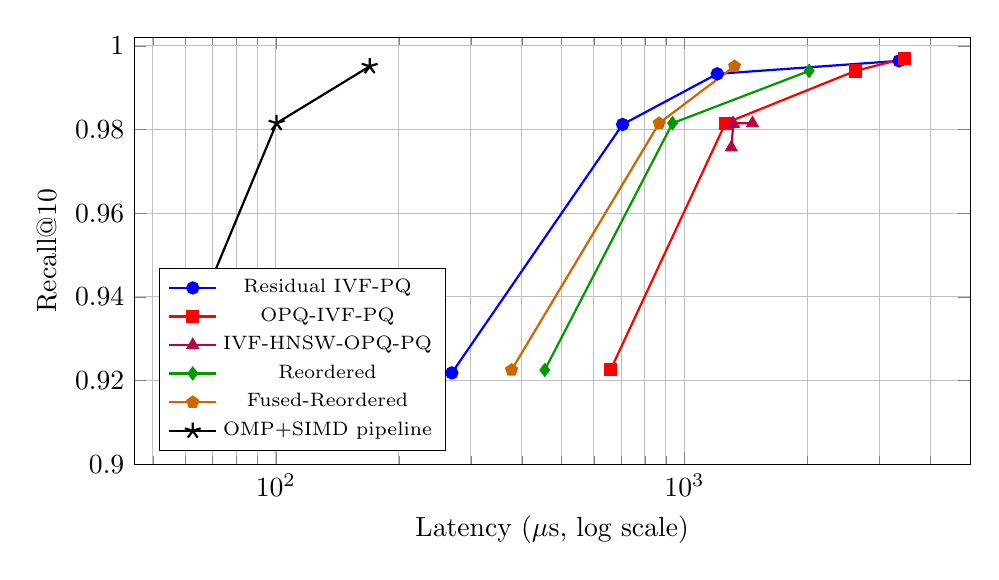
\begin{tikzpicture}
\begin{axis}[
    xlabel={Latency ($\mu$s, log scale)},
    ylabel={Recall@10},
    xmode=log,
    xmin=45, xmax=5000,
    ymin=0.90, ymax=1.002,
    grid=both,
    width=12.2cm,
    height=7cm,
    legend style={at={(0.03,0.03)},anchor=south west,font=\scriptsize}
]
\addplot[color=blue, mark=*, thick] coordinates {
    (269.621,0.921800) (705.421,0.981200) (1202.733,0.993300) (3349.157,0.996400)
};
\addlegendentry{Residual IVF-PQ}
\addplot[color=red, mark=square*, thick] coordinates {
    (659.751,0.922600) (1258.978,0.981500) (2617.980,0.994000) (3456.580,0.997000)
};
\addlegendentry{OPQ-IVF-PQ}
\addplot[color=purple, mark=triangle*, thick] coordinates {
    (1301.451,0.975700) (1316.535,0.981300) (1315.605,0.981500) (1466.597,0.981500)
};
\addlegendentry{IVF-HNSW-OPQ-PQ}
\addplot[color=green!60!black, mark=diamond*, thick] coordinates {
    (455.036,0.922500) (934.596,0.981500) (2017.852,0.994000)
};
\addlegendentry{Reordered}
\addplot[color=orange!80!black, mark=pentagon*, thick] coordinates {
    (377.489,0.922500) (866.680,0.981500) (1325.508,0.995100)
};
\addlegendentry{Fused-Reordered}
\addplot[color=black, mark=star, mark size=3pt, thick] coordinates {
    (56.301,0.922500) (100.417,0.981500) (169.710,0.995100)
};
\addlegendentry{OMP+SIMD pipeline}
\end{axis}
\end{tikzpicture}
\caption{A-E 多方案参数扫描的 Latency-Recall@10 Trade-off}
\label{fig:advanced-tradeoff}
\end{figure}

图\ref{fig:advanced-tradeoff}展示的是整组参数扫描，而不是单点速度对比。结合曲线形态，可以得到以下综合结论。
\begin{enumerate}
\item \textbf{Recall 的主导因素是候选覆盖，而不是某个单独算子的速度。} A、B、D、E 都随着 $nprobe$ 和 $R$ 增大从约 0.922 移动到 0.995 以上，说明只要候选桶覆盖足够、rerank 集合足够大，最终 top-$k$ 仍主要由精确 rerank 保证。0.98 以后曲线变平，说明此时错误主要来自少量近邻没有进入候选集合，需要付出大量额外候选扫描才能弥补。
\item \textbf{Latency 的主导因素是候选数据流，而不只是候选数量。} B 与 D 在 np16-R500 处的平均候选数几乎相同，recall 也同为 0.9815，但 B 的 latency 为 1258.978 $\mu$s，D-Reordered 为 934.596 $\mu$s，D-Fused 为 866.680 $\mu$s。这说明候选集合确定以后，内存布局、score 写回、top-$R$ 选择方式会直接决定端到端延迟。
\item \textbf{OPQ 与 HNSW 是结构性优化，必须与系统实现配套。} B 的 OPQ-lite 提高了量化空间均衡性，但在本实现中带来 permutation 访存代价；C 的 centroid graph routing 减少了完整扫描的理论需求，但 $nlist=64$ 时完整 centroid 扫描过于便宜，图扩展难以体现优势。因此二者更适合在更大 codebook、更强布局优化或更高维数据规模下释放收益。
\item \textbf{D 和 E 共同构成最终 Pareto 曲线左移的主要来源。} D 在单 query 内通过连续化和融合减少候选扫描阶段的中间内存流量，E 再把每条 query 的独立搜索映射到 OpenMP batch 并行。也就是说，第三部分不是简单把 IVF、PQ、HNSW 和 OpenMP 叠加，而是在候选生成、候选扫描、精排和批量执行四个层次逐步消除瓶颈。
\item \textbf{实际选型应按目标 recall 分段。} 若目标 Recall@10 约为 0.92，E 的 np8-R200 已能提供 56.301 $\mu$s/query 的最低延迟；若目标约为 0.98，E 的 np16-R500 是主要工作点；若目标接近 0.995，E 的 np24-R1000 保持高 recall，同时仍比单线程高召回 Fused 版本快 $7.81\times$。因此最终方案应优先选择满足 recall 下限的最小 $nprobe$ 与 $R$，而不是盲目追求最大参数。
\end{enumerate}

\subsection{性能分析}

profiling 不再对所有参数点重复展开，而是先从每个方案的参数扫描中选择代表点。选择原则是：在 Recall@10 不低于约 0.98 的主要工作区间内，取该方案 latency 最低的配置；D 组同时保留 Reordered 和 Fused-Reordered，用于直接观察数据重排与算子融合的增量；E 组为 OpenMP batch pipeline，表中 wall latency 是端到端批处理时间折算到单 query 的结果，而各阶段耗时是线程内部累计工作量，因此不能与 wall latency 简单相加。

\begin{table}[H]
\centering
\scriptsize
\caption{代表参数点查询阶段 profiling（$\mu$s/query）}
\label{tab:advanced-profile}
\begin{tabularx}{\textwidth}{Xrrrrrr}
\toprule
方案代表点 & Wall latency & Routing & LUT & PQ scan / fused top-$R$ & Unfused top-$R$ & Exact rerank \\
\midrule
A Residual np16-R500 & 705.421 & 6.968 & 45.524 & 456.878 & 118.889 & 77.161 \\
B OPQ np16-R500 & 1258.978 & 12.954 & 89.595 & 829.369 & 198.301 & 128.759 \\
C IVF-HNSW ef48 & 1315.605 & 25.308 & 95.300 & 848.736 & 221.339 & 124.923 \\
D Reordered np16-R500 & 934.596 & 23.600 & 92.188 & 487.694 & 216.061 & 115.054 \\
D Fused np16-R500 & 866.680 & 26.299 & 104.966 & 617.948 & 0.000 & 117.467 \\
E Pipeline np16-R500 & 100.417 & 50.235 & 254.173 & 1534.792 & 0.000 & 298.318 \\
\bottomrule
\end{tabularx}
\end{table}

根据表\ref{tab:advanced-profile}，代表参数点的瓶颈可以分解为以下几类。
\begin{enumerate}
\item \textbf{A 的主要瓶颈是 PQ scan 与显式 top-$R$。} np16-R500 下，PQ scan 为 456.878 $\mu$s，显式 top-$R$ 为 118.889 $\mu$s，二者合计 575.767 $\mu$s，占 wall latency 的 81.6\%。这说明残差 PQ 已经把精确 rerank 压到 77.161 $\mu$s，但粗排阶段仍需要对约 2.4 万候选写出 approximate score，并再做一次 top-$R$ 选择。因此 A 的瓶颈不是浮点内积本身，而是“压缩候选得分生成 + 候选筛选”的内存流。
\item \textbf{B 的瓶颈说明 OPQ-lite 需要与布局共同设计。} OPQ-lite 让 recall 略有提高，但 routing、LUT、PQ scan、top-$R$ 和 rerank 全部增加，其中 PQ scan 达到 829.369 $\mu$s。其原因在于维度 permutation 改善了子空间方差分配，却让查询 residual、LUT 构造和 code 累加的访问顺序更不连续；同时更高质量的 PQ 粗排会把更多相近候选推入 top-$R$，rerank 阶段也更容易访问分散的原始向量。该现象表明量化误差降低和硬件友好访问并不是天然一致的目标。
\item \textbf{C 的瓶颈说明 centroid graph 在小 $nlist$ 下不是关键路径。} C 的 routing 为 25.308 $\mu$s，高于 A/B 的完整 centroid 选择阶段；PQ scan 和 top-$R$ 仍分别为 848.736 $\mu$s 与 221.339 $\mu$s，接近 B 的主要耗时。因此在 $nlist=64$ 时，图路由减少的 centroid 计算不足以覆盖堆扩展、邻接访问和分支判断成本。它更像一个面向大规模 $nlist$ 的结构预研，而不是当前数据规模下的直接加速点。
\item \textbf{D-Reordered 证明了数据重排对 cache locality 的直接价值。} Reordered 不改变候选集合，却把 B/C 中非连续的 list 访问转为 list 内连续扫描，使 PQ scan 从 829--849 $\mu$s 降到 487.694 $\mu$s。这个下降不能用 recall 或候选数解释，只能由数据布局解释：同一倒排桶内的 ID、code 和 vector 连续存放后，预取更稳定，cache line 利用率更高，扫描阶段不再频繁跨桶随机跳转。
\item \textbf{D-Fused 证明了算子融合的收益来自减少中间结果，而不是减少每个候选的算术量。} Fused 后 ``PQ scan / fused top-$R$'' 为 617.948 $\mu$s，高于 Reordered 的纯 PQ scan；但显式 top-$R$ 从 216.061 $\mu$s 变为 0，wall latency 从 934.596 $\mu$s 降到 866.680 $\mu$s。也就是说，融合后的单次扫描内部多了堆维护判断，但避免了完整 score 数组写回、第二次遍历和 nth-element 选择，端到端更快。
\end{enumerate}

\begin{figure}[H]
\centering
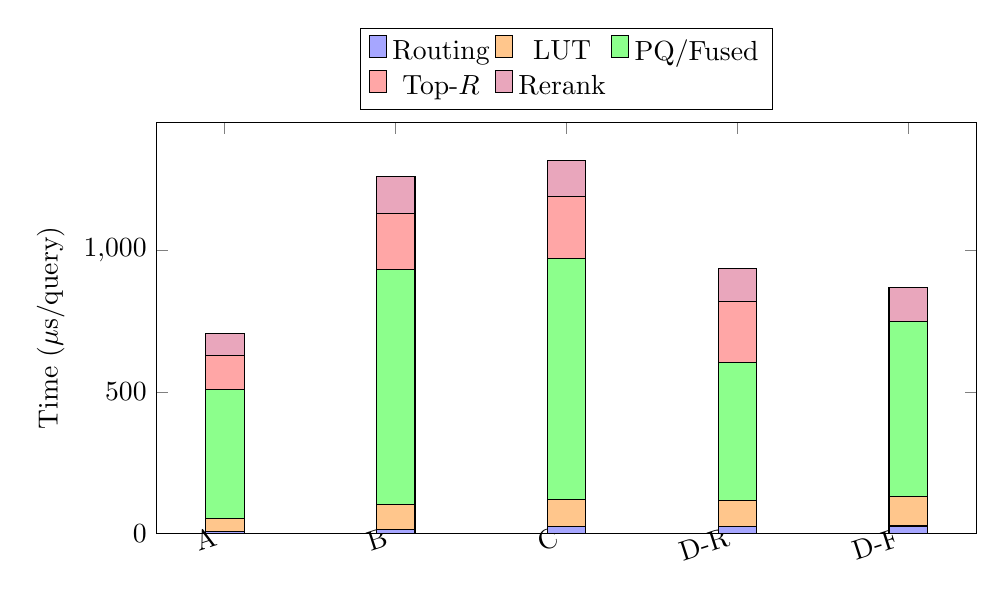
\begin{tikzpicture}
\begin{axis}[
    ybar stacked,
    ylabel={Time ($\mu$s/query)},
    symbolic x coords={A,B,C,D-R,D-F},
    xtick=data,
    width=12cm,
    height=6.8cm,
    ymin=0,
    ymax=1450,
    bar width=14pt,
    legend style={at={(0.5,1.03)},anchor=south,legend columns=3},
    nodes near coords={},
    x tick label style={rotate=18,anchor=east}
]
\addplot[fill=blue!35] coordinates {(A,6.968) (B,12.954) (C,25.308) (D-R,23.600) (D-F,26.299)};
\addlegendentry{Routing}
\addplot[fill=orange!45] coordinates {(A,45.524) (B,89.595) (C,95.300) (D-R,92.188) (D-F,104.966)};
\addlegendentry{LUT}
\addplot[fill=green!45] coordinates {(A,456.878) (B,829.369) (C,848.736) (D-R,487.694) (D-F,617.948)};
\addlegendentry{PQ/Fused}
\addplot[fill=red!35] coordinates {(A,118.889) (B,198.301) (C,221.339) (D-R,216.061) (D-F,0.000)};
\addlegendentry{Top-$R$}
\addplot[fill=purple!35] coordinates {(A,77.161) (B,128.759) (C,124.923) (D-R,115.054) (D-F,117.467)};
\addlegendentry{Rerank}
\end{axis}
\end{tikzpicture}
\caption{A-D 代表参数点查询耗时构成}
\label{fig:advanced-profile}
\end{figure}

\begin{table}[H]
\centering
\small
\caption{Pipeline-OMP-SIMD 相对单线程 Fused-Reordered 的吞吐提升}
\label{tab:pipeline-speedup}
\begin{tabular}{lrrrr}
\toprule
参数点 & Recall@10 & Fused latency & Pipeline latency & Speedup \\
\midrule
np8-R200 & 0.922500 & 377.489 & 56.301 & $6.70\times$ \\
np16-R500 & 0.981500 & 866.680 & 100.417 & $8.63\times$ \\
np24-R1000 & 0.995100 & 1325.508 & 169.710 & $7.81\times$ \\
\bottomrule
\end{tabular}
\end{table}

结合图\ref{fig:advanced-profile}和表\ref{tab:pipeline-speedup}，profiling 的综合结论如下。
\begin{enumerate}
\item \textbf{E 组的 profiling 不能与 A-D 直接相加比较。} A-D 是单 query 串行路径上的阶段分解，阶段时间之和接近 wall latency；E 是多 query 并行执行后的 wall-time latency，表中 route、LUT、scan、rerank 是线程内部累计工作量，不代表单条 query 的串行路径。因此 E 的核心指标应看 wall latency、QPS 和相对单线程 Fused 的 speedup。
\item \textbf{query-level 并行是当前 CPU 上更稳定的并行粒度。} 在 i7-14650HX 的 24 逻辑线程环境下，E 在 np8、np16、np24 三个参数点分别获得 $6.70\times$、$8.63\times$、$7.81\times$ 加速，且 recall 完全不变。加速比没有达到 24 倍，主要来自三类限制：不同 query 命中的倒排桶大小不同导致负载不均；每条 query 内仍有堆维护和随机 rerank 访问；候选扫描阶段受内存带宽与 cache 行为限制，不能随线程数线性缩短。
\item \textbf{算法参数与性能瓶颈之间存在明确因果关系。} $nprobe$ 和 $R$ 增大时 recall 上升，是因为更多真实近邻进入 rerank 集合；同时 latency 上升，是因为 PQ scan、top-$R$ 维护和 exact rerank 都随候选规模扩大。$ef$ 增大时 recall 先上升后饱和，是因为 graph routing 的 coarse 漏召回被修复后，继续扩展只增加图访问成本。OPQ-lite 让量化空间更均衡，但如果不配合连续布局，会把瓶颈从量化误差转移到 permutation 访存。
\item \textbf{最终有效组合可以概括为候选压缩、连续布局、算子融合、批量并行。} IVF/PQ 先把全库搜索压缩成局部候选扫描；Reordered 把局部候选改造成硬件更容易连续读取的数据流；Fused 把 score 生成和 top-$R$ 筛选合并，减少中间数组；Pipeline-OMP-SIMD 再把多条独立 query 分配给线程，并在每条 query 的 rerank 中保留 AVX2/FMA。四个层次分别对应算法剪枝、数据重排、算子融合和硬件并行，缺少任一层都会留下明显瓶颈。
\item \textbf{异构协同的合理边界应由 profiling 决定。} 结合前面 GPU Compact 实验，GPU 最适合处理 compact candidate pair 的批量 scoring，而不适合直接承担分支密集的 HNSW routing 与小粒度堆扩展。更合理的路线是 CPU 负责 centroid graph routing、倒排桶组织和 batch 调度，GPU 接收已经压缩好的候选 pair，在设备端完成局部 top-$R$/top-$k$，只回传少量候选结果，从而避免完整距离矩阵和大规模 D2H 传输。
\item \textbf{构建开销不是本规模下的主要矛盾。} Residual-IVF-PQ 总构建时间为 0.170500 s，OPQ-lite-IVF-PQ 为 0.186618 s，其中 OPQ-lite 维度重排仅 0.002708 s，远小于 coarse assignment、PQ 训练、PQ 编码和倒排重排。因此在 DEEP100K 规模下，进阶方案的主要取舍发生在在线查询阶段；若扩展到百万级以上，KMeans、PQ 编码和重排会成为离线成本，但只要索引用于大量查询，构建开销仍可被摊销。
\end{enumerate}

\section{总结与收获}

通过 ANNS 选题对并行程序设计的系统实践，我最深的体会是：并行优化不能只理解为“把循环并行化”或“把代码搬到 GPU 上”，而是要先判断问题中的数据依赖、访存模式、候选规模和硬件执行粒度是否匹配。ANNS 查询表面上是向量距离计算问题，但随着算法从 Flat 扫描发展到 IVF、PQ、HNSW 和 GPU Compact，真正决定性能的因素逐渐从单次内积吞吐转向候选生成质量、倒排表访问局部性、top-$k$ 维护开销、CPU/GPU 之间的数据传输规模以及 batch 调度方式。因此，可靠的并行程序设计需要同时回答三个问题：哪些工作可以独立并行，哪些数据值得搬运，哪些中间结果应当尽量避免产生。

从 SIMD、OpenMP/Pthread、MPI 到 GPU 的实验过程也让我更清楚地理解了不同并行层次的边界。SIMD 适合处理向量维度内部规则、连续的计算；OpenMP/Pthread 更适合 query 级或候选集合级共享内存并行；MPI 适合数据分片后的跨进程协同，但必须关注通信、负载均衡和全局 top-$k$ 合并；GPU 适合大批量、规则化的 scoring kernel，但如果候选展开方式导致无效 pair 过多或 D2H 回传过大，端到端性能并不会自然变好。第三部分的进阶实验进一步说明，真正有效的优化往往来自多层次组合：先用索引结构减少候选，再用数据重排改善访存，再用算子融合减少中间数组，最后再选择合适的并行粒度提升吞吐。

本报告中的平时工作主要包括：ANNS 基础流程理解、DEEP100K 数据读取与 ground truth 评估、Flat/SIMD 距离计算、OpenMP/Pthread 共享内存并行、MPI 数据分片、GPU batch/compact 实验，以及 IVF、PQ、HNSW 等基础算法和对应的 latency-recall、profiling 分析。期末新增工作主要包括：在平时实验基础上重新整理完整 ANNS 系统流程；横向融合 SIMD、OpenMP、MPI、GPU 与 Flat、IVF、PQ、HNSW 的对比；新增 Residual-IVF-PQ-Rerank、OPQ-lite-IVF-PQ、IVF-HNSW-OPQ-PQ、Reordered/Fused IVF-HNSW-OPQ-PQ 和 Pipeline-OMP-SIMD 五组进阶实验；补充多参数扫描、Latency-Recall@10 trade-off、阶段 profiling、流程图和关键伪代码，并分析算子融合、数据重排和硬件协同对性能的影响。

本报告相关代码与结果已整理到 GitHub 仓库：
\begin{center}
\scriptsize\url{https://github.com/liuyuze-121/NKU-cpu-parallel-lab/tree/main/lab_final_programming}
\end{center}

\end{document}
